\chapter{半导体应用指南：把 Part 11 读成一条证据链}

\begin{noteblock}
Semantica 边界： 本附录保留 Part 11 的可读解释、来源坐标叙述、算例与建模
蓝图；它不在书内发布本体、查询、Shape 或 runner。现有
\nolinkurl{semantica.chapter_packages.vol2.ch06}、\nolinkurl{vol2.ch16}、\nolinkurl{vol2.ch18} 分别承接度量、
测量证据和依赖主题的章级机器合同，但当前 Semantica registry 尚无“Part 11 全附录”
的独立 released package。本附录中的形式化片段因此只是书面蓝图；若要执行，必须先
作为显式 Semantica package delta 注册、补齐 CQ/正反例/oracle/来源与 release 证据，
未注册前一律视为 unsupported/blocked，不能回退到旧本地文件。
\end{noteblock}

\begin{noteblock}
\textbf{导读}。正文各章把 ISO 26262 的生命周期走了一遍，芯片在其中大多以“某个元件、某个失效率”的面目一闪而过。本附录面向想深入半导体功能安全的读者，把 ISO 26262-11:2018（下称 Part 11）组织成一条“对象划分\(\rightarrow\)基础失效率\(\rightarrow\)相关失效分析\(\rightarrow\)故障注入\(\rightarrow\)具体技术案例”的证据链。读完本附录，你应当能：
1. 拿到一颗芯片或一个 IP，说清它在 component/part/subpart 层次里的位置、失效模式与故障模型如何挂接，以及 IP 供需双方各自欠对方什么工作产物；
2. 面对一个“XX FIT”的基础失效率，追问并核对它的来源、任务剖面、置信水平与适用边界，手算复核 Part 11 自带的示例；
3. 用 DFI 七分类和 B1–B12 工作流组织一次半导体相关失效分析，并说清哪些结论可以量化、哪些只能定性留证。

\textbf{来源性质声明（先读）}：Part 11 全卷为\textbf{资料性（informative）}。其 Scope 明说“This document has an informative character only. It contains possible interpretations of other parts of ISO 26262 with respect to semiconductor development”（Part 11 物理页 p9）。也就是说，本附录中的 Part 11 内容是对 ISO 26262 其他分册在半导体开发中的可能解释，\textbf{不构成新的规范性要求，也不能替代任何适用的 shall}。凡本附录说“可以这样算/这样分类”，Part 11 锚点只支撑这一解释的来源归属；需要形成项目义务时，须逐项回到适用的规范性条款（主要位于 Parts 2–9，术语还需回看 Part 1），或显式标成 \nolinkurl{BookHousePolicy}/\nolinkurl{ProjectSpecificStrategy}，不能靠 Part 11 单独升级。

\textbf{标签边界}：带 ISO 条款/表格锚点的陈述才可作为“标准事实”候选，且还要区分 shall、NOTE 与 EXAMPLE；“本书归纳/本书建议”是\textbf{作者综合}；\nolinkurl{TeachingExample} 是合成教学数据；\nolinkurl{BookHousePolicy} 是本书的证据接收或知识治理规则；\nolinkurl{ProjectSpecificStrategy} 是具体项目的选择。五者不得互相代替。

\textbf{案例边界}：本附录引用的数值多数是 Part 11 自带的计算示例；关键数值与 A.8 的来源坐标曾用两种同源提取视图定位，并回看原 PDF。后文简写的“两源核对”均只表示这两种提取视图一致，不表示存在两个独立来源。本附录自行补充的算例一律标注“教学示例”（\nolinkurl{TeachingExample}），不代表任何真实器件的失效率或量产结论。页码为 1-based 物理页。

\textbf{与全书二十章的衔接}：本书前十章现为叙事重写，方法表语义、独立性等级记号、FMEDA 与失效分类等器具性内容已集中由附录承载；正文各章只提供活动与主题的工程语境。本附录因此按自足深讲编写——凡指向“第 X 章”处均指主题语境，不意味着正文有逐表逐条的展开。
\end{noteblock}


\Needspace{6\baselineskip}
\section{导读：芯片不是一只黑盒}

先讲一个会真实发生的场景。某整车项目的系统安全团队按第 6 章讲过的流程做硬件度量：技术安全需求分配到了电子控制单元，FMEDA——第 6 章展开过的失效模式、影响及诊断分析——排到了主控芯片这一行。芯片是外购的：一颗集成了 CPU、存储器、模数转换器和若干通信外设的车规微控制器，其中还嵌着一块第三方授权的处理器核。团队手里只有一份功能数据手册：引脚定义、电气参数、外设清单，一应俱全；但要填进 FMEDA 的三样东西——失效率怎么分到内部模块、每个模块坏了算哪类故障、片内自检覆盖到什么程度——手册上一个字都没有。芯片对他们来说是一只黑盒，而定量分析恰恰要求把盒子打开。

这个困境不是哪家公司管理不善，而是半导体供应链的结构性事实。整车厂不设计芯片，芯片厂不了解整车安全目标，芯片里还嵌着第三方的设计模块；分析所需的信息分散在链条各处，谁也无法独自完成论证。Part 11 就是为这个断层写的说明书。它把断层拆成四个可以逐个处理的问题：

\textbf{第一，划分粒度}。芯片内部要拆到多细才能做分析？拆浅了失效模式挂不上诊断，拆深了几百万门根本算不动。Part 11 §4.2 给出 component\(\rightarrow\)part\(\rightarrow\)subpart\(\rightarrow\)elementary subpart 的层次词汇，并明说粒度取决于安全概念与所用的安全机制（p10）——这是 A.2 节的主题。

\textbf{第二，使用假设}。芯片厂做分析时并不知道你的系统长什么样，只能假设“用户会这样用我”。这类假设有个专名：先记白话版——“我按你会给我配软件驱动、会把我的报错引脚接到监控器来设计”这类前提；正式名是\textbf{使用假设}（Assumptions of Use, AoU）。Part 11 §4.1.1 与 §4.4 资料性地描述了把 AoU 写出并在更高集成层级核对的做法（p10、p13）；当元素按 SEooC 裁剪时，真正的 shall 在 Part 2 §6.4.5.7：开发须基于预期使用与上下文假设，集成进目标应用时须验证这些假设。假设不核对，芯片级分析的漂亮数字到了系统级就是空中楼阁——A.2 节的 ECC 软件驱动反例会演示这一点。

\textbf{第三，证据可见性}。IP 供应商未必愿意、也未必被允许交出设计细节；极端情况是加密网表或混淆源码的“黑盒 IP”。看不见内部时，谁来估失效率、谁来定义外部安全机制？Part 11 §4.5.5 的资料性回答是：用\textbf{开发接口协议}——第 10 章深讲过的 DIA（Development Interface Agreement），明确责任、可交付证据与接受边界（p22–23）。DIA 是 ISO 26262 的分布式开发接口工件；它在某个司法辖区是否同时构成法律合同，不由 Part 11 这几个示例决定。

\textbf{第四，责任划分}。半导体开发者在供应链里既是供应商又是客户；确认措施、生产控制、现场监控这些正文 ch03/ch09 讲过的义务，落到芯片上要怎么裁剪？A.6 节沿 §4.9–§4.12 走一遍。

本附录的路线与正文的回指关系如下表：

\begin{center}
\begingroup\small
\setlength{\tabcolsep}{4pt}
\begin{tabularx}{\linewidth}{@{}XXXX@{}}
\toprule
节 & Part 11 素材 & 物理页 & 回指正文 \\
\midrule
A.2 部件划分、故障模型与 IP 边界 & §4.1–§4.5 & p10–23 & 第 2 章概念层次、第 10 章 SEooC/DIA \\
A.3 基础失效率 & §4.6 & p23–49 & 第 6 章 \(\lambda\) 分类与 FMEDA 输入链 \\
A.4 半导体 DFA & §4.7 & p49–63 & 第 8 章 DFA 与独立性 \\
A.5 故障注入 & §4.8 & p63–65 & 第 5/6 章验证计划与覆盖率主张 \\
A.6 生产、分布式开发与确认 & §4.9–§4.12 & p65–68 & 第 9 章生产、第 10 章 DIA、第 3 章确认措施 \\
A.7 五类技术案例 & §5.1–§5.5 & p68–140 & 各技术章 \\
A.8 本体化实践 & 全部锚点 & — & 第 6 章数值诚实、第 8 章依赖链 \\
\bottomrule
\end{tabularx}
\endgroup
\end{center}

怎么读一卷“资料性”标准，也值得先说破。informative 不等于没有工程价值：Part 11 集中给出了诸多把 Parts 2–9 应用到半导体开发的解释与示例，在相关评审、审计或供应链沟通中可作为参考；但它也不等于照抄即合规。原文常用“can be used”“is recommended”“a rationale is provided”这类表达，选择与论证仍要回到具体上下文。本书的阅读策略（作者综合）是：把方法当作\textbf{候选}，把 NOTE 当作\textbf{解释与边界信息}，把数值示例当作\textbf{练习题的参考答案}而不是项目数据。本附录因而说“Part 11 建议/示例”，不说“Part 11 要求”。

一句话立骨：\textbf{正文教你要什么证据，本附录教你这些证据在硅片上长什么样}。

\Needspace{6\baselineskip}
\section{半导体部件划分、故障模型与 IP 边界}

\Needspace{5\baselineskip}
\subsection{四层划分：分析粒度是安全概念的函数}

第 2 章讲过的 element 层次词汇——item/system/component/part——在芯片内部继续向下延伸。Part 11 §4.2 按 Part 1 §3.21 的定义给出示范：整颗半导体是 \textbf{component}；第二层级（例如一个 CPU）是 \textbf{part}；再往下（例如 CPU 的寄存器组）是 \textbf{subpart}；直到\textbf{基本子部件}（elementary subpart，例如寄存器组里的单个寄存器及其相关逻辑，或一个触发器、一只模拟晶体管）（p10，Figure 2 见 p11）。

关键不在名词，而在紧随其后的那条 NOTE：\textbf{拆到哪一层、“基本子部件”取什么颗粒，取决于安全概念、分析所处阶段与所用的安全机制}（p10）。这句话是全附录反复回响的主旋律。两个对照例子（§4.3.2，p12）：同一个 CPU，若安全机制是硬件锁步——两个核逐拍比对输出——对该机制所覆盖的 CPU 内部故障，失效模式可以在“CPU 功能整体”这一层定义；这不表示锁步能发现所有内部或共因故障。若安全机制换成软件自检程序，为得到可辩护的诊断覆盖率通常需要拆细，因为自检对不同内部结构的覆盖率不同。\textbf{机制越“包圆”，划分可以越粗；机制越“挑食”，可信分析所需的划分通常越细}。这是 Part 11 的分析指南，不是独立的粒度 shall。

\Needspace{5\baselineskip}
\subsection{故障模型、失效模式与“无缝隙”检查}

第 2 章讲过的 fault\(\rightarrow\)error\(\rightarrow\)failure 因果链在芯片语境里落地为两个衔接的概念。\textbf{故障模型}（fault model）是物理故障的抽象表示（§4.3.1，p11）：晶体管栅氧击穿、金属互连断裂这些物理事件数不胜数，工程上把它们归并为“节点恒为 0/1（stuck-at）”“开路”“桥接”这类可枚举、可注入、可统计的模型。\textbf{失效模式}（failure mode）则描述功能层面“怎么坏”：Part 11 建议用关键词法——错误的程序流、数据损坏、访问了不该访问的位置、死锁、活锁、错误指令执行（§4.3.2 EXAMPLE 4，p12）。

\begin{figure}[htbp]
\centering
\adjustbox{max size={\linewidth}{0.78\textheight}}{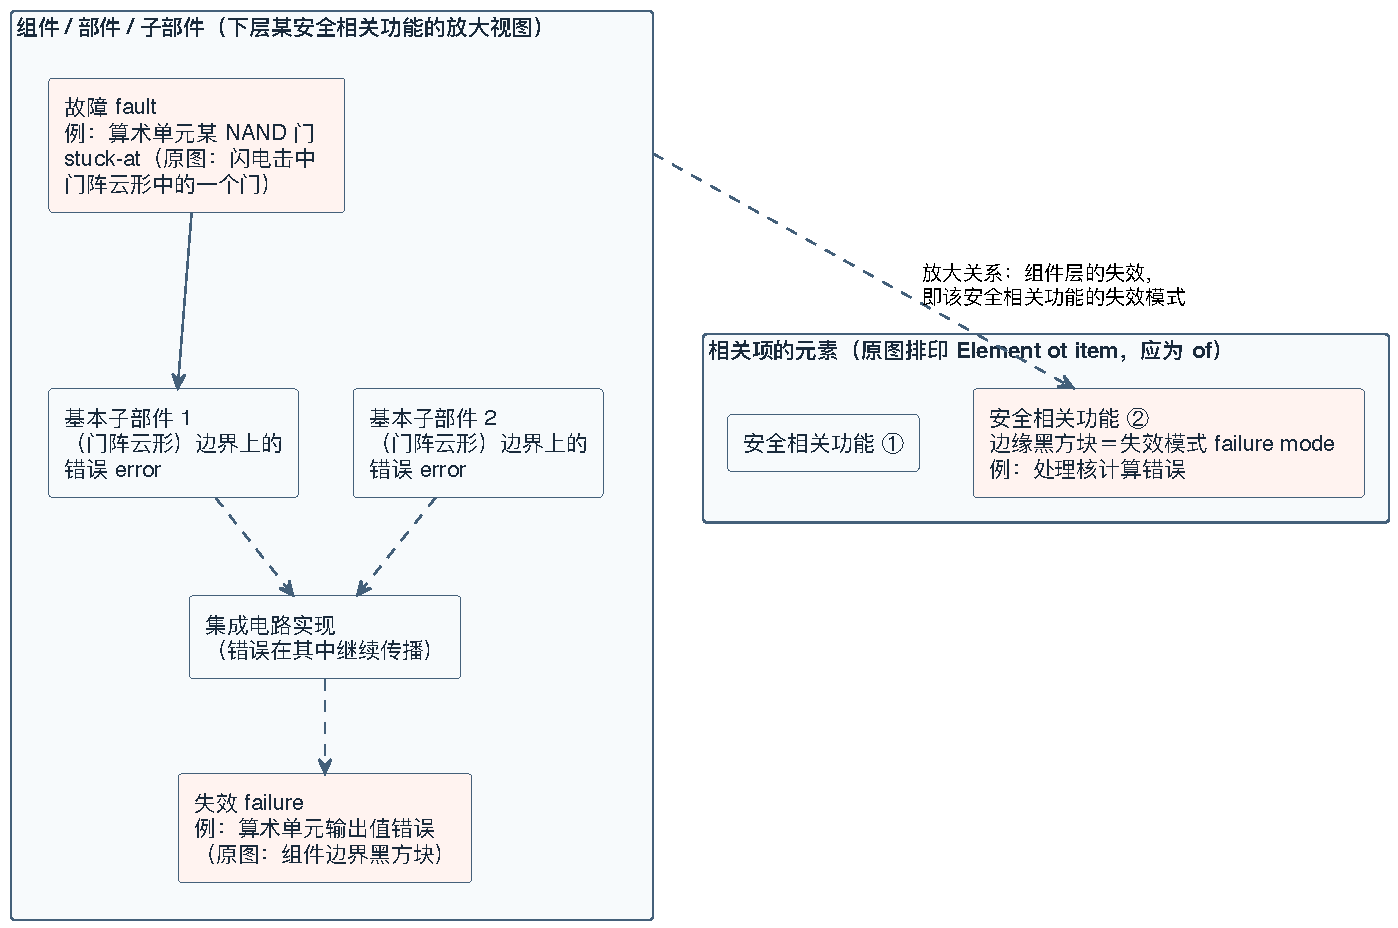
\includegraphics{figures-rendered/appA-fig1-p11-figure3-fault-failure-mode.pdf}}
\setcounter{figure}{0}
\caption{硬件故障与失效模式的关系（重绘自 Part 11 Figure 3）——基本子部件内的物理故障在子部件边界成为错误、经集成电路实现传播为组件层失效；同一失效在相关项元素层即某安全相关功能的失效模式，两层由放大关系相连。}
\end{figure}

两者的挂接关系直接决定诊断覆盖率怎么算。§4.3.1 的示例值得手算一遍（p12）：若某失效模式由 stuck-at 故障贡献 X\%、由短路贡献 Y\%，而安全机制只覆盖 stuck-at 且覆盖率为 Z\%，则可主张的诊断覆盖率是 X\% \(\times\) Z\%。代入具体数（教学示例）：stuck-at 占 70\%、短路占 30\%、机制对 stuck-at 覆盖 90\%，则总覆盖率是 0.7 \(\times\) 0.9 = 63\%，而不是 90\%——短路那 30\% 完全在机制视野之外。\textbf{当局部覆盖率只针对某个故障模型子集时，总体主张必须按该子集对相关失效模式的贡献加权}；不能把局部 Z\% 直接写成总体 Z\%。这是本书审阅半导体安全手册时采用的一把尺。

§4.3.2 还给出一项“无缝隙”完整性指南（p12）：用证据支撑失效模式与电路实现的关联，检查\textbf{每个失效模式都分配到某个 part/subpart，每个相关的 part/subpart 至少有一个失效模式}。目的写得很直白：确保电路实现与失效模式清单之间没有缝隙。这与第 6 章 FMEDA 的完整性纪律同构——那里防“漏元件”，这里防“漏模块”。本书把这项资料性指南采纳为审稿/接收策略时，规则依据应标成 \nolinkurl{BookHousePolicy}，不能标成 \nolinkurl{DirectISORequirement}。

失效率往失效模式上摊时（§4.3.3，p12），精度同样跟着安全机制走：锁步 CPU 不需要精细分布，软件自检 CPU 需要。没有数据支撑分布时，Part 11 给出两条资料性做法——均匀分布，或给出带论证的专家判断——并在 NOTE 中建议做\textbf{敏感性分析}，看分布假设对诊断覆盖率与定量结果的影响有多大。退路不是免费的：均匀分布省了测量，就得用敏感性分析补充对结论稳健性的认识；若项目把它设为放行条件，应另标 \nolinkurl{BookHousePolicy}。

\Needspace{5\baselineskip}
\subsection{从芯片级到系统级：自底向上与假设核销}

§4.4 回答“芯片级细粒度分析如何对接系统级粗粒度分析”（p13）。方向一：把芯片的详细失效模式\textbf{自底向上}归并成系统分析需要的高层失效模式（Figure 4），自顶向下的 FTA 与自底向上的 FMEA 在中间会师；从低抽象层出发的好处是失效分布可以定量而非拍脑袋（NOTE 2）。方向二：诊断覆盖率可以在更高层级\textbf{被改善}——芯片里一个没有任何硬件安全机制的模数转换器，孤立看覆盖率为零；到了系统级它被纳入闭环，软件一致性检查能发现它的故障，覆盖率随之上升（EXAMPLE 1）。

方向三是最容易翻车的：芯片级覆盖率可能建立在特定使用假设之上。§4.4 的 EXAMPLE 2（p13）是个教科书级反例：某芯片的存储器带 ECC，单比特错误可纠正并向 CPU 报告；芯片级分析\textbf{假设}用户会实现一个软件驱动来处理这个报告事件。系统集成时，出于性能考虑这个驱动没做——假设失效，芯片被改配置为把纠错标志直接甩到片外。此时芯片安全手册里那一行漂亮的覆盖率数字已经不再成立。\textbf{AoU 不是参考资料，是待核销的债务清单}：在 SEooC 场景，逐条验证的规范依据是 Part 2 §6.4.5.7 b)；本书再用 \nolinkurl{BookHousePolicy} 把核销结果固定成“满足/不满足/替代措施”三态，避免只继承结论不继承前提。

\Needspace{5\baselineskip}
\subsection{IP：四条路径、两种类别、一套工作产物}

\textbf{IP} 在 Part 11 里指打算作为 part 或 component 集成进设计的可复用逻辑或物理设计单元；提供方叫 IP 供应商，集成方叫 IP 集成者——两者可以是不同公司，也可以是同一公司的两个部门（§4.5.1.1，p14）。按交付形态分两类（Table 1，p15）：\textbf{硬 IP}（物理表示：完整版图，如 ADC 宏、PLL 宏）与\textbf{软 IP}（模型表示：Verilog/VHDL 或晶体管级原理图，还要经过综合、布局布线才成为硅上实现）。这个区分有安全后果，A.2.5 会用到：对尚未确定最终工艺与物理实现的软 IP，失效率与分布只能先作为基于实现假设的参考估计，并由集成者对具体实现重新核对（§4.5.4.5 NOTE 1，p20）。

基于 ISO 26262 的既有机制，Part 11 识别出 IP 进入安全设计的\textbf{四条路径}（§4.5.3，Figure 5，p14、p17–19）：

\begin{center}
\begingroup\small
\setlength{\tabcolsep}{4pt}
\begin{tabularx}{\linewidth}{@{}XXXX@{}}
\toprule
路径 & 依据 & 适用场景 & 集成者的核对重点 \\
\midrule
SEooC 开发 & Part 10（ch10 深讲） & IP 面向一类假想上下文开发 & 逐条验证 AoU 与实际上下文一致 \\
在上下文中开发 & Part 2 §6.4.5.1 & 供需双方同项目协作，安全需求已知 & 常规分布式开发管理 \\
硬件元素评估 & Part 8 Clause 13 & 无 SEooC/在场信息的既有 IP & 按评估程序补置信 \\
在用验证（proven in use） & Part 8 Clause 14 & 有大规模现场历史 & 现场监控与配置一致性论证 \\
\bottomrule
\end{tabularx}
\endgroup
\end{center}

第四条路的门槛被 Part 11 特意泼了冷水（§4.5.3.5，p19）：IP 的现场反馈通常很有限、配置又千差万别，Part 8 §14.4.5.3 要求的有效现场监控计划很难满足——\textbf{“用了很多年”不等于“在用验证成立”}。

按安全需求分配情况，Part 11 §4.5.2 资料性地区分两种 IP（p15）：\textbf{未分配安全需求}的 IP 通常不因 Part 11 自身增加事项；若安全分析识别出它会影响安全相关元素，适用的 Part 9 Clause 6/7 要求仍需处理。\textbf{分配了安全需求}的 IP 则根据具体上下文裁剪并适用 Parts 2/4/5/8/9 的相应要求，再按“是否内建安全机制”细分（Figure 6，p16）。内建机制的 IP（例如带内建总线监督器的总线 fabric、带过压/欠压监控和自诊断的电压调节器）可以主张对特定失效模式的覆盖；无机制的 IP（同样的 fabric/调节器裸奔版）通常只能给出失效模式清单与分布，把覆盖论证留给集成层。类别划分来自 Part 11 指南，具体义务来自被判定适用的 Parts 2–9 条款。

还有两类“生成物 IP”值得单独说。\textbf{可配置 IP}：逻辑设计形态的 IP 常带配置选项——总线位宽、存储容量、中断数量、是否例化故障检测机制——配置由集成者指定（§4.5.1.2 NOTE 1，p15）。配置不是无害的开关：§4.5.4.5 资料性地说明，可配置 IP 的安全分析可描述配置选项对失效模式分布的影响，其 NOTE 3 还提到对安全机制实现与诊断覆盖率的影响分析（p20）；§4.5.3.2 又说明 SEooC IP 供应商提供\textbf{哪些配置已被测试与验证活动覆盖}的信息（p19）。若所选组合不在该信息范围内，本书的证据接收策略（\nolinkurl{BookHousePolicy}）把覆盖率主张视为待重新论证，而不是自动继承。顺带一条 NOTE：IP 配置不同于软件的配置数据，Part 6 Annex C 不直接适用于 IP（§4.5.3.2 NOTE 1，p19）。\textbf{工具生成的 IP}（存储编译器、C 转 HDL 编译器、片上网络生成器）：对生成工具的信任可按 Part 8 Clause 11 的软件工具置信度框架处理，并结合对生成 IP 的验证程度裁剪\textbf{工具鉴定}活动；生成结果本身的正确性验证则由适用的供需方分工，例如写入 DIA（§4.5.1.2 NOTE 2，p15）。

SEooC 路径还有一个“能力不匹配”的局面（§4.5.3.2，p18）：IP 的 SEooC ASIL 能力（按 Part 1 §3.2）低于集成者的 ASIL 要求。Part 11 资料性地给出两条候选路径：集成者在 IP 外部追加安全机制、并补充系统性失效避免措施；或者按 Part 9 Clause 5 做 ASIL 分解——但要论证冗余安全需求及充分独立性，并把集成 IP 的系统性失效避免与控制方法一并纳入考虑。这与第 8 章的边界一致：缺少独立性证据时，不能据此主张 ASIL 分解成立。

对应地，§4.5.4.10 给出按类别裁剪工作产物的资料性解释（p22）：对无内建机制的 IP，安全分析信息可聚焦失效模式分布——没有机制就谈不上由该 IP 自身提供硬件度量估算；集成文档集可缩减为集成环境假设与接口说明；相关失效分析是否需要则取决于共存与依赖。\textbf{类别影响证据范围，但不由 Part 11 单独创造或免除义务}——审阅 IP 交付包时先判类别，再回到适用的 Parts 2–9 条款与 DIA 对清单。

Part 11 给出的 IP 工作产物指南（§4.5.4，p19–22）包括：安全计划、分配到 IP 的硬件安全需求、设计验证与验证评审、安全分析报告（定性给失效模式，定量给失效率与分布估计，配置类 IP 还可分析配置选项对分布与机制覆盖的影响）、相关失效分析、确认措施结果（安全计划/安全分析/安全档案完整性的确认评审、审核与评估报告——回指第 3 章的确认措施框架）、DIA，以及\textbf{集成文档集}。§4.5.4.9 说明这些信息可合并为一册\textbf{安全手册}（Safety Manual）或安全应用笔记，内容包括：生命周期裁剪说明、AoU（假定安全状态、最大故障处理时间与多点故障检测间隔假设、集成环境与接口假设、推荐配置）、安全架构描述（故障检测/控制/报告/自检/恢复机制及配置参数影响）、支撑安全机制所需的硬件-软件接口、片上故障软件测试例程规格、安全分析结果与确认措施说明（p21–22）。两条资料性 NOTE 值得画线：基础失效率\textbf{只能作为参考值}提供，因为它取决于 IP 在集成电路中的实际实现工艺与使用条件，NOTE 4 将按实际用例重算的责任指向 IP 集成者（§4.5.2，p17）；NOTE 1 则说明 IP 安全机制需求应以可追溯到集成者需求的方式表达（§4.5.4.9，p22）。这两句是 Part 11 的指南，不是新增 shall。

\Needspace{5\baselineskip}
\subsection{黑盒 IP：看不见内部时，责任写进 DIA}

有时集成者被要求集成一个内容不披露的 IP：客户的专有通信接口逻辑、竞争对手的模块（为了多源供货协议）。交付形态可能是预硬化版图、加密网表或混淆 RTL（§4.5.5，p22）。此时，基于内部结构的分析会受限，但外部测试、集成指南与外部安全机制并未因此失效。Part 11 的资料性对策是通过 DIA \textbf{明确 IP 供应商、IP 集成者与集成者客户之间的责任划分与证据交换}（p23）。DIA 可以约定：由客户负责评估并接受黑盒 IP 在安全上下文中的适用性（EXAMPLE 3）；由供应商提供含验证测试集的集成指南（EXAMPLE 4）；当 IP 不是按 ISO 26262 开发（例如按 IEC 61508）时，由谁负责接受可用证据（EXAMPLE 5 与 NOTE 2 的差距分析）。基础失效率同理：集成者不一定拥有足够数据估算黑盒 IP 的失效率，Part 11 建议在 DIA 中识别估算责任（p23）；若需要外部安全机制而集成者信息不足，也可在 DIA 中约定由谁给出相应需求。DIA 相关项目义务的规范性来源是适用的 Part 8 Clause 5，而不是 Part 11 的示例措辞。

一句收口（作者综合）：\textbf{看得见的 IP 用内部证据集成，看不见的 IP 则把证据缺口与责任边界写清}。本书的 \nolinkurl{BookHousePolicy} 不允许黑盒状态把未分配责任默认成“无人处理”。

\Needspace{6\baselineskip}
\section{基础失效率：来源、假设与计算边界}

\Needspace{5\baselineskip}
\subsection{基础失效率是什么，不是什么}

第 6 章的 FMEDA 输入链里，每一行的起点都是一个 \(\lambda\)。那个 \(\lambda\) 的学名在 Part 11 里叫\textbf{基础失效率}（base failure rate，也叫 raw failure rate）：元件在\textbf{没有任何安全机制干预之前}的固有随机硬件失效率，是 Part 5 定量分析与度量计算的首要输入（§4.6.1.1，p23）。单位沿用第 6 章讲过的 FIT：1 FIT = 10\(^{-9}\) 次/小时。

三条边界先划清楚。\textbf{其一，只算随机，不算系统性}（§4.6.1.3，p24）。多数可靠性预计技术不区分两者，结果可能因掺入系统性因素而过度保守；有些模型甚至内置“过程质量因子”（如 FIDES 的 \(\pi\)\_pm、\(\pi\)\_process），这些因子对应系统性能力，在 ISO 26262 语境下要剥离——A.3.4 的 FIDES 示例正是把它们置 1。\textbf{其二，不与诊断混算}（§4.6.1.4，p24）。一个反直觉的例子：带单纠双检 ECC 的 SRAM，厂商报出的平均无故障时间（MTTF）通常不把“可纠正错误”算作失效——这等于把基础失效率与诊断效果搅在了一起，而 Part 5 的度量计算要求两者分开：\(\lambda\) 是 \(\lambda\)，覆盖率是覆盖率，先分后乘。\textbf{其三，PMHF 目标值不是可靠性预计输入}（§4.6.1.2，p24）。第 6 章讲过的 PMHF 随机硬件失效概率度量，其量化目标值按 Part 5 §9.4.2.2 NOTE 1 只有相对意义——用于新旧设计对比与设计引导——不能拿去“倒推”元件该有多可靠。

还有一条埋得深但杀伤力大的假设：\textbf{常数失效率}（§4.6.1.5，p25）。标准化模型普遍采用“浴盆曲线”简化——早夭段已被供应商筛选剪除、磨损段（电迁移、时变介质击穿、热载流子、负偏压温度不稳定性）在任务寿命内可忽略，只剩平底段的常数 \(\lambda\)。若可靠性模型给出的分布不满足常数假设，Part 5 的架构度量算法就不兼容；出路是取分布的最大值做保守常数近似，或限制产品运行寿命使常数近似成立（EXAMPLE 1/2）。NOTE 1 提醒：如果指数模型下产品寿命内会走到浴盆尽头并超出失效率目标，那是一个\textbf{系统性问题}，其可接受性不在 Part 5 Clause 8/9 的硬件度量中评价，而要单独评估；原文举的一种证据是按 AEC-Q100 完成的集成电路\textbf{鉴定（qualification）}结果（p25）。更准确地说，Clause 8/9 度量使用常数失效率近似；早期失效与磨损机理还需在度量之外另行评估，不能笼统地说成“交给认证就结束”。

\Needspace{5\baselineskip}
\subsection{四类来源与配套假设}

估基础失效率的技术分四族（§4.6.1.6，p26）：

\begin{enumerate}
\item \textbf{实验测试}：高温工作寿命试验（HTOL/TBOL/ELT）、工艺可靠性测试芯片与片上测试结构、辐射源暴露的软错误测试（JESD89 给方法）、筛选加速试验的收敛特性；
\item \textbf{现场数据}：退货失效品分析折算，A.3.5 详述；
\item \textbf{工业数据手册}：IEC 61709、SN 29500、FIDES Guide、以及“电子元件可靠性预计模型”（前 IEC TR 62380）——注意 NOTE 3 的方向感：实际达到的失效率\textbf{预期低于}手册推出的值，手册天生偏保守；
\item \textbf{路线图投影}：IRDS/ITRS 对各工艺代软错误率的投影值，可作首次估计，待工艺实测数据到位后再精化。
\end{enumerate}

不同技术对失效机理的假设不同，\textbf{未经机理与应力口径对齐的两个失效率不能直接比较}（§4.6.1.1，p23–24）——同一颗芯片用两种手册算出不同结果，可能是各自计入的机理集合与应力假设不同，不能先验地判定某一方错误。调和（harmonization）的做法原文给了方向：考虑同一组失效机理与同一组应力来源（EXAMPLE 1，p24）。本书将它操作化为 \nolinkurl{BookHousePolicy}：先列出各来源计入的机理清单（氧化层击穿？电迁移？焊点疲劳？软错误？），再对齐应力假设（结温、循环幅度、湿度）；只比较口径可对齐的部分，其余差异要么补测，要么显式声明为暂不可比。Part 11 还建议参考 JEDEC、IRDS、SEMATECH/ISMI 等行业组织的出版物获取机理级认识（p24）。

正因来源五花八门，§4.6.1.7 给出一份\textbf{假设文档化指南}（p26–27）：随失效率说明选用的方法（手册还是现场数据）、假定的任务剖面、数据的置信水平、施加过的缩放或降额、非工作时间与焊点如何计入、现场数据用的是威布尔还是指数模型。这份清单是集成者在元素或相关项层面评价、比较乃至\textbf{调和}不同供应商失效率的重要抓手。本书把“缺少这份清单就不接受 FIT 值”设为 \nolinkurl{BookHousePolicy}；这是证据接收策略，不是 Part 11 产生的 shall。把它类比成第 6 章的说法：\textbf{没有假设清单的 FIT 值，等于没有量纲的数字}。

瞬态故障的量化有专门指南（§4.6.1.8，p27–28）。由内外部 \(\alpha\)、\(\beta\)、中子、\(\gamma\) 辐射引发的软错误属于随机硬件失效，可用测量数据支撑的概率方法量化；对电磁干扰或串扰引发的瞬态，Part 11 建议不走随机硬件量化，而按主要为系统性成因处理。它也建议把瞬态与永久故障分开分析，并逐类基本子部件（触发器、锁存器、存储单元、模拟器件）排查软错误敏感性；封装材料也参与其中——低 \(\alpha\)（LA）/超低 \(\alpha\)（ULA）封装材料能改变 \(\alpha\) 粒子致错率（EXAMPLE 1）。三条防“注水”提醒同样属于资料性解释：不要只按整车运行时间摊薄软错误基础失效率（EXAMPLE 2）；不要预先用架构脆弱性因子（AVF）或 ECC 效果降额——脆弱性因子属于安全故障占比的账，在 5.1.7.2 里算；若交付的是降额后软错误率，应在安全手册中披露降额因子（NOTE 4–6）。本书将这三项设为数据接收 \nolinkurl{BookHousePolicy}，才使用“不得混账/必须披露”的门禁语气。

封装的账目归属要小心（§4.6.1.9，p28）：芯片厂的失效率覆盖裸片、封装外壳与连接点（引脚），而\textbf{引脚到电路板的焊点}通常算板级失效、由系统集成者在系统或元素层分析。三种手册的口径不一样：前 IEC TR 62380 模型的 \(\lambda_{\mathrm{package}}\) 把焊点也包了进去；SN 29500-2 的元件失效率含裸片与封装但不含焊点（焊点另见 SN 29500-5）；FIDES 则把外壳与焊点分开给。\textbf{跨手册比较前，先对齐“封装”一词的边界}。

\Needspace{5\baselineskip}
\subsection{手册路线之一：前 IEC TR 62380 模型的完整走查}

Part 11 §4.6.2.1.1 以前 IEC TR 62380 为底本给出一套完整模型（p28–38）：\(\lambda\) = 裸片项 + 封装项 + 过应力项。裸片项的参数：每晶体管失效率 \(\lambda\)\(_{1}\)（按电路族查表）、工艺掌握度失效率 \(\lambda\)\(_{2}\)（整片一个值）、晶体管数 N、工艺年代降额指数 \(\alpha\)（与参考年 1998 的年差）、工作/储存时间比 \(\tau\)\_i/\(\tau\)\_on/\(\tau\)\_off、结温应力因子 (\(\pi\)\_t)\_i；封装项的参数：热膨胀失配因子 \(\pi\)\_\(\alpha\)（板材 \(\alpha\)\_s 与封装 \(\alpha\)\_c 之差）、年热循环数与幅度 (n\_i, \(\Delta\)T\_i)、封装基础失效率 \(\lambda\)\(_{3}\)（按引脚数 S 或封装对角线 D 查表）；过应力项：接口暴露因子 \(\pi\)\_I 与环境过应力率 \(\lambda_{\mathrm{EOS}}\)（p29）。

\textbf{裸片示例手算}（Table 2，p34；数值两源核对一致）。一颗 CMOS 微控制器：5 万门 CPU（每门 4 管，N = 200 000）与 16 kB SRAM（低功耗 SRAM 每位 6 管，N = 786 432），功耗 0.5 W，144 脚四方扁平封装自然对流散热，“电机控制”温度剖面下结温升 \(\Delta\)T\_j = 26.27 \(^{\circ}\)C，激活能 0.3 eV，温度降额因子算得 0.17。CPU 行：\(\lambda\)\(_{1}\) = 3.4\(\times\)10\(^{-6}\) FIT/管，\(\lambda\)\(_{1}\)·N = 0.68 FIT；工艺年代项 e\^{}(-0.35\(\times\)10) \(\approx\) 0.030，得 0.021 FIT；加上按晶体管数加权的 \(\lambda\)\(_{2}\) 份额 (200 000/986 432)\(\times\)1.7 \(\approx\) 0.345 FIT，乘降额 0.17 \(\approx\) \textbf{0.06 FIT}。SRAM 行：1.7\(\times\)10\(^{-7}\)\(\times\)786 432 \(\approx\) 0.134，\(\times\)0.030 \(\approx\) 0.004；加权 \(\lambda\)\(_{2}\) 份额 (786 432/986 432)\(\times\)8.8 \(\approx\) 7.02，乘 0.17 \(\approx\) \textbf{1.18 FIT}。合计裸片失效率 \textbf{1.25 FIT}——与表中一致。读表提醒：Table 2 的“Base failure rate”列印的是 \(\lambda\)\(_{1}\) 项加\textbf{未加权}的整值 \(\lambda\)\(_{2}\)（1.73/8.80），而“Effective”列按加权公式算，两列口径不同，抄表时容易踩坑。若嫌加权麻烦，Table 5（p36）给了粗粒度算法：整片按同一电路族计算，\(\lambda\)\(_{1}\)·N·e\^{}(-3.5) \(\approx\) 0.10，加 \(\lambda\)\(_{2}\) = 1.7 得 1.80，乘 0.17 得 \textbf{0.31 FIT}——在该示例中比逐元素算保守。混合信号的对应处理见 Table 3（p34）：\(\lambda\)\(_{2}\) 取各族\textbf{最大值}做保守合并（示例结果 3.44 FIT）；BiCMOS 三元素的完整逐步计算（式 (3)–(17)，p35–36）最终 \(\lambda_{\mathrm{die}}\) \(\approx\) 2.01 FIT，其中 \(\lambda\)\(_{2}\) 相关项 2.01 FIT 远大于 \(\lambda\)\(_{1}\) 相关项 6.05\(\times\)10\(^{-4}\) FIT——\textbf{在这个 BiCMOS 示例中，工艺掌握度项是主导项}；不应把这一示例直接外推到所有模拟工艺。

走完这个示例，把模型的温度降额参数摊开看一眼（§4.6.2.1.1.2，p36）：(\(\pi\)\_t)\_i 是任务剖面第 i 个相位的结温应力因子，\(\tau\)\_i 是该相位的工作时间比，\(\tau\)\_on = \(\sum\)\(\tau\)\_i 是总工作时间比，\(\tau\)\_off 是储存（或休眠）时间比，两者之和恒为 1。降额因子 = \(\sum\)(\(\pi\)\_t)\_i·\(\tau\)\_i / (\(\tau\)\_on + \(\tau\)\_off)。BiCMOS 示例的中间步骤展示了它怎么算（式 (4)–(7)，p35）：三个温度相位（32/60/85 \(^{\circ}\)C）各自按 Arrhenius 式算出 \(\pi\)\_t 再乘时间比，加和得 8.25\(\times\)10\(^{-2}\)——\textbf{任务剖面就是这样一相位一相位地进入失效率的}。也因此，本书的 \nolinkurl{BookHousePolicy} 把剖面里每一行“多少小时、什么温度”的出处列为 §4.6.1.7 假设清单的必填项。

\textbf{降额因子的方向感}（§4.6.2.1.1.2，p36–37）：\(\tau\)\_off 是储存时间比，\(\tau\)\_on + \(\tau\)\_off = 1。保守做法是令 \(\tau\)\_off = 0（只按工作相位算），示例里降额因子从 0.17 变 2.91，有效失效率从 0.31 FIT 涨到 \textbf{5.24 FIT}——差 17 倍。这个示例显示，任务剖面里“车停着不通电”的时间占比可以改变结论量级，这正是假设文档化纪律有工程价值的理由。

\textbf{封装示例}（Table 6，p37）：PQFP 144，FR4 基板 \(\alpha\)\_s = 16 与塑封 \(\alpha\)\_c = 21.5 得 \(\pi\)\_\(\alpha\) = 1.05，按 0.5 mm 间距、20 mm 边宽查 \(\lambda\)\(_{3}\) = 11.87 FIT，热循环项中间量 6 009（模型内部的无量纲量，随年循环数与温幅进入公式），含焊点的封装失效率 206 FIT；按“焊点约占 20\%”的经验扣除后 \textbf{\(\lambda_{\mathrm{package}}\) = 166 FIT}（20\% 粗算为 164.8，表值 166 的差来自查表取整）。按引脚均摊：166/144 \(\approx\) \textbf{1.15 FIT/脚}（手算核对：166 \(\div\) 144 = 1.153）。NOTE 3 提醒均摊不总是成立——BGA 某些位置的分布更高（p38）。

\textbf{过应力项}（§4.6.2.1.1.4，p38）：模型没有汽车电气环境的 \(\lambda_{\mathrm{EOS}}\)，示例借“民用航电（机载计算机）”的 20 FIT；器件直连外部环境（是接口）则 \(\pi\)\_I = 1、\(\lambda_{\mathrm{overstress}}\) = 20 FIT，否则为 0。NOTE 又把门打开了一半：电气过应力可视为系统性失效模式，在随机硬件度量计算中降为 0 FIT——前提是你论证并缓解了它的系统性成因，而不是当它不存在。

\Needspace{5\baselineskip}
\subsection{手册路线之二与三：SN 29500 与 FIDES}

\textbf{SN 29500} 走查表路线（§4.6.2.1.2，p38–41）：按产品类型、工艺、晶体管数查参考条件下的 \(\lambda_{\mathrm{ref}}\)，再用修正的 Arrhenius 方程折算到实际工作条件（温度、电压、漂移）。表格没有你的规格时允许插值：示例中 50 万门微控制器落在 CMOS 表 10 万门（76 FIT@80 \(^{\circ}\)C 虚拟结温）与 100 万门（80 FIT@90 \(^{\circ}\)C）之间，先把各列折算到同一虚拟参考温度 90 \(^{\circ}\)C，线性插值得 \(\lambda_{\mathrm{ref}}\)(500K@90 \(^{\circ}\)C) = 78.2 FIT，虚拟结温插值得 84.4 \(^{\circ}\)C，再回折得 \textbf{62 FIT}（p39）。套上“电机控制”任务剖面（年工作 500 小时、三档环境温度加权）得总温度因子 \(\pi\)\_T = 1.31，整片有效失效率 \(\approx\) \textbf{105 FIT}（Table 8，p40）。与 62380 模型的口径差异：SN 29500 默认\textbf{只算工作小时}，非工作相位要额外乘应力因子 \(\pi\)\_w——示例中按全球昼夜均温 10.5 \(^{\circ}\)C 算得 \(\pi\)\_w = 0.06，104.65 FIT 折到含非工作相位的 \textbf{6.3 FIT}（Table 9，p41；手算核对 104.65 \(\times\) 0.06 = 6.28 \(\approx\) 6.3）。同一颗芯片，“每工作小时”与“每日历小时”两种单位差 17 倍——\textbf{单位口径是 §4.6.1.7 建议披露的事项，也是本书数据接收 \nolinkurl{BookHousePolicy} 的必填项}。SN 29500 整值不拆裸片/封装，需要拆分时按专家判断，例如借用 62380 的比例（§4.6.2.1.2.4，p41）。

\textbf{FIDES Guide} 路线（§4.6.2.1.3，p41–44）：失效率 = 物理贡献 \(\lambda_{\mathrm{Physical}}\) \(\times\)过程贡献 \(\pi\)\_Process \(\times\) 制造贡献 \(\pi\)\_PM。后两个因子对应系统性问题，Part 11 的 ISO 26262 计算示例将它们\textbf{置 1}。物理贡献覆盖热、温度循环、机械、湿度四族应力（示例为简化只算前两族）。示例数值：裸片 \(\lambda\)\_0TH 合计 0.13 FIT（CPU 0.08 + SRAM 0.06），简化任务剖面下温度降额 5.79，裸片有效 \textbf{0.75 FIT}；细化任务剖面（增加满载、高速公路等相位）降额升到 12.44，裸片有效 \textbf{1.61 FIT}（Table 13/16，p43–44）。\textbf{在这个示例中}，剖面细化后结果约翻一倍，说明任务剖面可能是高敏感输入，但不证明它在所有模型和项目中都排第一。封装（含循环降额）0.25 FIT；焊点 0.12 FIT 仅供参考、不计入封装。

三条手册路线并排看的教学结论：62380 模型、SN 29500、FIDES 对同一颗教学芯片给出的失效率分别在 1.25（裸片）、105（整片，每工作小时口径）/6.3（整片，含非工作）、0.75–1.61（裸片）FIT 量级——注意 SN 29500 的整值不拆裸片/封装，这三组数连口径都不同层。这些差异主要提醒读者核对模型边界、失效机理集、任务剖面和小时口径；不能只用“假设不同”解释一切差异，也不能从三个示例中选一个当作真值。本书建议选定有适用性理由的路线、写全假设、在整个项目里保持口径一致，并在与供应商数据对表时先做机理与口径调和。

\Needspace{5\baselineskip}
\subsection{现场数据路线与实验路线}

现场数据看似最“真”，实则最需要戒心（§4.6.2.2，p44–45）。先审流程三问：已知质量问题在退货流程中怎么处理的？真实任务剖面知道多少？现场监控的有效性如何？Part 2 §7.4.2.3 的 shall 是组织建立、执行并维护生产/运行/服务/退役阶段的功能安全过程，其 NOTE 说明这包括现场监控；Part 11 再资料性地建议半导体供应商关注数据收集、上置信限、系统性故障剔除条件、\textbf{修正因子}（CF）理由，以及经验证模型给出的\textbf{加速因子}（AF）。本书把这些建议转成现场数据接收清单时标记为 \nolinkurl{BookHousePolicy}，不把整张清单冒充 Part 2 原句。

计算用指数模型加卡方统计（§4.6.2.2.1，p45）：FIT = \(\chi\)\(^{2}\)(CL; 2n+2) \(\times\) 10\(^{9}\) / (2 \(\times\) 累计运行小时 \(\times\) AF)，其中 n 为失效数乘修正因子；Part 11 建议使用至少 70\% 置信水平的单侧上置信限。原文把它口语化为“真实失效率有 70\% 概率低于该值”，但频率学上更严谨的解释是：\textbf{若在固定真值下反复按同一抽样与构造程序求上限，至少约 70\% 的上限会覆盖该真值}；不能把固定真值说成在本次区间内具有 70\% 的后验概率。示例（§4.6.2.2.2，p45–47）：三款在役芯片的任务剖面折算出等效结温（55.1/51.4/67.4 \(^{\circ}\)C），用 0.3 eV 激活能的 Arrhenius 折到参考温度 55 \(^{\circ}\)C，合计裸片面积小时 805 317 百万 mm\(^{2}\)·小时；保修期失效 4 起，乘 CF = 5 得 20 起，卡方 70\% 上界折算得 \textbf{0.029 FIT/mm\(^{2}\)}（Table 19，p46）。新设计芯片 23 mm\(^{2}\)、等效结温 75 \(^{\circ}\)C、加速因子 1.84：0.029 \(\times\) 1.84 \(\approx\) 0.053 FIT/mm\(^{2}\)，\(\times\)23 \(\approx\) 1.23，与表值 \textbf{1.22 FIT} 的微小出入来自表内中间值修约（Table 20，p47；表列 FIT/mm\(^{2}\) 修约为 0.05）。封装失效率同法，但加速因子换 Coffin-Manson 或 Norris-Landzberg 模型（NOTE 4）。

加速寿命试验路线（§4.6.2.3，p47–48）：从试验温度降额到最高工作温度用 0.7 eV 激活能的 Arrhenius（原文建议对目标失效机理估计并验证激活能）；样本失效数经卡方分布外推到总体；CMOS 还要考虑电压加速。此处有一个值得保留的源文疑点：Part 11 式 (25) 在原 PDF 与提取视图中均排印为 \allowbreak{}\texttt{AF\_\allowbreak{}v \allowbreak{}=\allowbreak{} \allowbreak{}exp(\(\beta\)) \allowbreak{}\(\times\) \allowbreak{}[V\_\allowbreak{}t \allowbreak{}- \allowbreak{}V\_\allowbreak{}o]}\allowbreak{}，同页又把 \(\beta\) 的单位写成 \nolinkurl{1/V}，因而按量纲检查存在疑点。本附录忠实记录该排印，但不把它当作可直接执行的计算式；项目应回到所选可靠性模型的受控公式与参数定义核对。

\Needspace{5\baselineskip}
\subsection{失效率的再分配与多芯片模块}

算出整片失效率后，还要摊到组成元素的失效模式上（§4.6.2.4，p48）。裸片部分两法：\textbf{按面积}——失效率密度（FIT/mm\(^{2}\)）乘以该 part/subpart 的占用面积（Part 11 §5.1.7.1 的例子：CPU 占裸片面积 3\%，就摊总失效率的 3\%）；\textbf{按门数}——基本子部件（门/晶体管）失效率乘以数量。封装部分：有封装失效率时按“总失效率 \(\div\) 总引脚数”得每脚失效率，再按安全相关引脚分摊。选哪种方法看版图信息可得性与失效模式在硬件元素间的共享方式（NOTE）。多芯片模块（MCM）单列一条（§4.6.2.5，p49）：Part 11 建议套用工业手册时给出适用性或定制理由——手册的统计基础通常是单芯片封装，多裸片互连的失效机理未必被覆盖；本书将该理由设为接收条件时标记为 \nolinkurl{BookHousePolicy}。

\Needspace{5\baselineskip}
\subsection{选路线的决策清单}

四条路线不是并列的自助餐，各有前置条件。给一张教学用的决策清单（本表为本书归纳，非 Part 11 原文表格；最后一列是 \nolinkurl{BookHousePolicy}，不是 ISO shall）：

\begin{center}
\begingroup\small
\setlength{\tabcolsep}{4pt}
\begin{tabularx}{\linewidth}{@{}XXXX@{}}
\toprule
你手里有什么 & 优先路线 & 主要风险 & 本书接收策略要求的补充说明 \\
\midrule
只有设计规格与工艺信息 & 工业手册（62380 模型 / SN 29500 / FIDES） & 模型结果往往偏保守，但仍需验证机理集与应力的适用性 & 手册版本、参数选择理由、口径（工作/日历小时） \\
同工艺同封装的量产历史 & 现场数据 + \(\chi\)\(^{2}\) 上界 & 退货流程失真、任务剖面未知 & CF 修正因子理由、监控有效性、剖面文档 \\
新工艺、无历史 & 加速寿命试验 / 可靠性测试芯片 & 激活能假设与目标机理不符会显著扭曲外推 & 目标机理的激活能实测验证 \\
深亚微米软错误 & JESD89 测量 + IRDS 投影过渡 & 投影值只是首次估计 & 拿到工艺实测后更新，标注中子通量/海拔等条件 \\
\bottomrule
\end{tabularx}
\endgroup
\end{center}

\begin{sidewaysfigure}
\centering
\adjustbox{max size={0.92\textheight}{0.85\textwidth}}{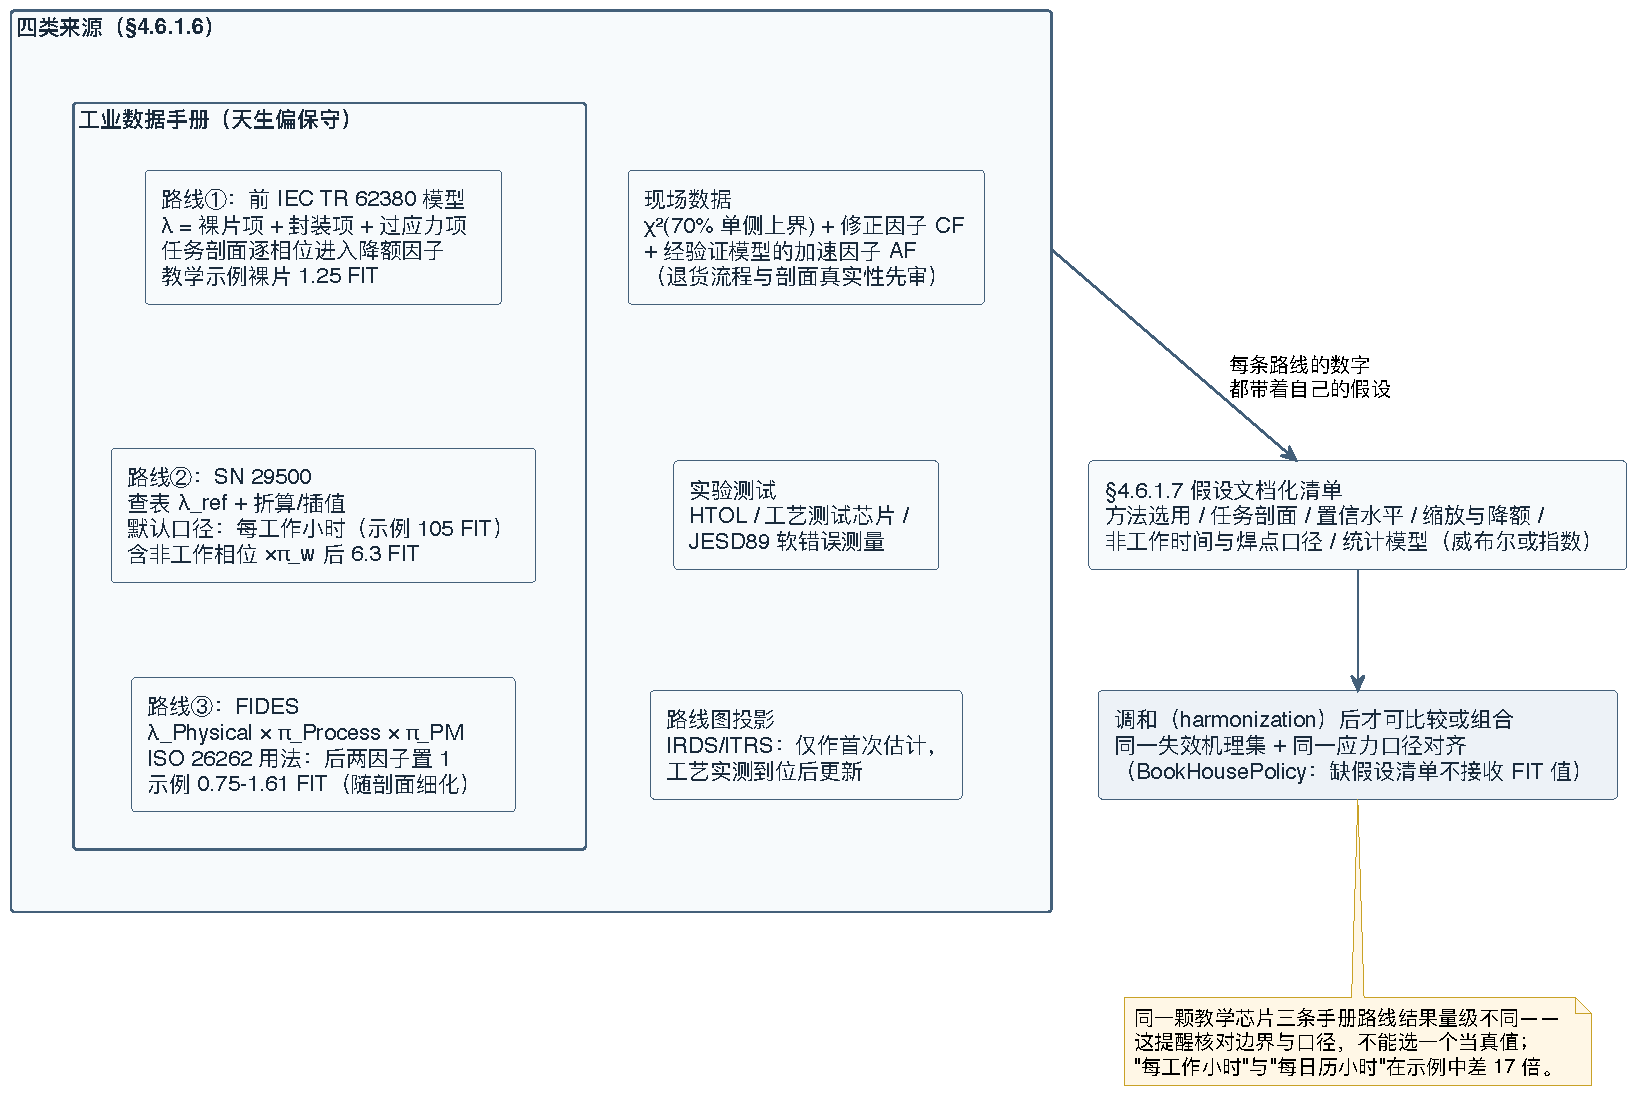
\includegraphics{figures-rendered/appA-fig2-base-failure-rate-routes.pdf}}
\setcounter{figure}{1}
\caption{基础失效率来源路线图——工业手册三条路线（前 IEC TR 62380 模型、SN 29500、FIDES）与现场数据、实验测试、路线图投影四类来源各带前置条件，全部汇入 §4.6.1.7 假设文档化清单；未经机理与口径调和的数字不进入比较与组合。}
\end{sidewaysfigure}

本书采用三条通用 \nolinkurl{BookHousePolicy}：\textbf{先调和，后组合或比较}——供应商 A 用现场数据、供应商 B 用 SN 29500 时，集成者按 §4.6.1.7 的假设清单对齐机理与口径，不直接把两个未调和的 FIT 值相加或比较；\textbf{声称保守就要验证方向}——对常数失效率、\(\lambda\)\(_{2}\) 取最大、\(\tau\)\_off 置零、70\% 上界等具体近似，逐一说明其为何不低估目标量，而不是笼统地声称“所有近似都保守”；\textbf{更新有触发器}——工艺、封装或任务剖面变更，以及获得足以改变估计的新现场数据时，启动失效率复核并保留版本链。

收口对仗：\textbf{来源给数字，假设给资格；口径不对齐，数字无意义}。这些纪律与第 6 章“数值诚实”的映射，在 A.8 节落成三元组。

\Needspace{6\baselineskip}
\section{半导体 DFA：DFI 七分类与 B1–B12 工作流}

\Needspace{5\baselineskip}
\subsection{为什么芯片内的相关失效要单独讲}

第 8 章首讲过相关失效分析——DFA（Dependent Failure Analysis），以及它服务的两大论证：ASIL 分解要求的\textbf{独立性}（Part 9 Clause 5）与共存分析要求的\textbf{免于干扰}（Part 9 Clause 6）。Part 11 §4.7 把镜头推近到\textbf{同一块硅片内部}：所有“独立”通道共享同一片衬底、同一套电源网络、同一棵时钟树、同一个封装——在系统层看似天各一方的元素，在芯片里可能只隔几微米。Part 11 §4.7 的范围声明就是这么写的：单一裸片内硬件元素之间、以及硬件与软件元素之间的 DFA（p49）。

核心术语沿用 Part 1 §3.30 的定义：\textbf{相关失效引发源}（Dependent Failure Initiator, DFI）——经由耦合因子导致多个元素失效的单一根因（p49）。这里要还一笔第 8 章挂过的账：Part 9 正文只说 root cause 与 coupling factor，\textbf{把 DFI 做成成体系分类的是 Part 11 §4.7.5.1}；Part 9 Annex C 表 C.1 最后一列的映射对象正是 Part 11 的这些 DFI 名。第 8 章的 DFA 九主题与七耦合因子是“分析什么”的清单，Part 11 的 DFI 七分类是“根因长什么样”的清单，两者是同一件事的两个切面。

DFA 与常规安全分析的分工（§4.7.1–§4.7.2，p49–50）：安全分析（Part 5 §7.4.3、Part 9 Clause 8）负责找单点/多点故障、算度量、定机制；DFA 补的是“机制的有效性会不会被相关失效掏空”。哪些元素需要 DFA，常常能从安全分析结果里直接读出来：\textbf{双点失效场景}——功能与其安全机制（含故障反应路径上的整条元素/任务链）、功能冗余（两路电流驱动器、两路 ADC）；\textbf{共享基础设施的单点（残余）场景}——时钟生成、嵌入式电压调节器、以及上述元素共用的任何硬件资源。Part 11 指南说明：已识别依赖关系且可按残余/单点/多点故障归类的随机硬件 DFI，可纳入 Part 5 Clause 8/9 的定量分析；不能可靠量化的系统性、环境性根因则继续定性处理（§4.7.3 NOTE 1，p51）。纳入度量不等于删除 DFA 追溯或自动闭环 Part 9 义务；本书的 \nolinkurl{BookHousePolicy} 仍要求保存依赖识别、分类与措施理由。

\Needspace{5\baselineskip}
\subsection{相关失效场景的解剖学}

§4.7.3（p50–52）给相关失效场景做了一次解剖，四个观察维度日后都会变成缓解措施的设计输入：

\begin{itemize}
\item \textbf{耦合机制}：根因如何把扰动送到受害元素——传导耦合（电或热，经导体直接接触）、近场耦合（容性=电场感应、感性=磁场感应，距离小于一个波长）、机械耦合（应力经物理介质传递——MEMS 的梳齿结构可能因特定共振冲击而粘连，专名 stiction，见 5.5.3.2）、辐射耦合（距离大于波长，源与受害者互为天线）；
\item \textbf{传播介质}：信号线、时钟网络、电源网络、衬底、封装、空气；
\item \textbf{局部性}：扰动是同时打击多个元素，还是只打击一个、再由其错误输出\textbf{级联}到下游；
\item \textbf{时间特征}：传播延迟（如温度梯度）、周期性（如电源纹波）。
\end{itemize}

这四个维度不只是分类，还可成为措施设计的输入表。本书的操作化示意是：传导耦合可考虑电气隔离与独立供电域，容性/感性近场耦合可考虑间距与屏蔽，机械耦合可考虑阻尼与结构设计，辐射耦合可考虑屏蔽与滤波；走电源、衬底或时钟网络的扰动，分别提示在电源域边界、物理隔离结构或时钟监督处寻找候选防线；局部性用于区分共因与级联传播；时间特征用于设计监控带宽和采样策略。这些都只是\textbf{候选手段}，不是某类耦合的唯一处方，也不自动证明措施足够。§4.7.5.2 资料性地建议论证“措施与目标 DFI 相称”；本书把四维逐项对表作为 \nolinkurl{BookHousePolicy} 的一种操作化，而不是 Part 11 的独立要求。

两张示意图值得记住（Figure 21/22，p52–53）。图 21：元素 A1 与 A2 冗余，比较器 B 检查输出——若同一根因让 A1、A2 产生\textbf{相同}的错误输出，B 在比对时刻无法分辨；只要两路错误存在时间或空间上的差异（扰动传播路径不同、时序违例效应不同），依赖场景仍可控（NOTE 2）——这正是后文“影响多样化”类措施的原理。图 22：共享元素 X 出错，错误输出同时馈入 A1 与 A2——“共享资源”类 DFI 的标准像。

级联失效与共因失效的区分，Part 11 §4.7.4 给出一个务实的资料性解释（p53）：对某些半导体分析，精确区分可能不可行或对分析目的没有增益，此时指南认为可不再细分。这不是对 Part 9 Clause 7 的普遍豁免；是否合并取决于项目能否仍满足所需独立性或免于干扰论证。若分析目的聚焦两个元素间的免于干扰，指南示例的四步是：找出元素 A 会影响 B 的失效模式\(\rightarrow\)判断这些模式是否经 B 的失效导致安全目标违背\(\rightarrow\)必要时定义缓解措施（例如给 DMA 配一个地址监控安全机制）\(\rightarrow\)\textbf{换位重做一遍}。

\Needspace{5\baselineskip}
\subsection{DFI 七分类与缓解措施两分法}

§4.7.5.1（p53–58）给出 DFI 的七个类别——这是本书第 8 章预告过的“DFI 七分类”的原文出处：

\begin{enumerate}
\item \textbf{共享资源失效}（随机硬件，Table 21，p55）；
\item \textbf{单一物理根因}（随机硬件，Table 22，p56）；
\item \textbf{环境条件}（系统性，Table 23，p56）；
\item \textbf{开发故障}（系统性，Table 24，p57）；
\item \textbf{制造故障}（系统性，Table 25，p57）；
\item \textbf{安装故障}（系统性，Table 26，p58）；
\item \textbf{服务故障}（系统性；对半导体元件通常为空集，理由见下段 NOTE 4）。
\end{enumerate}

NOTE 1 保留了开放性：其他分类法也可能适用（p54）。NOTE 4 解释了为什么第七类在半导体上通常是空集：汽车维修一般整体换 ECU 或传感器模块，半导体元件本身不被服务，所以服务故障通常不构成半导体的 DFI（p54）。NOTE 3 划了软件的界：软件引起的 DFI 不在此清单——正确的软件开发归 Part 6 管，但 DFA 的结果可以影响软件元素的 ASIL 分配（p54）。这些 NOTE 都是指南边界，不是封闭分类规则。

\begin{sidewaysfigure}
\centering
\adjustbox{max size={0.92\textheight}{0.85\textwidth}}{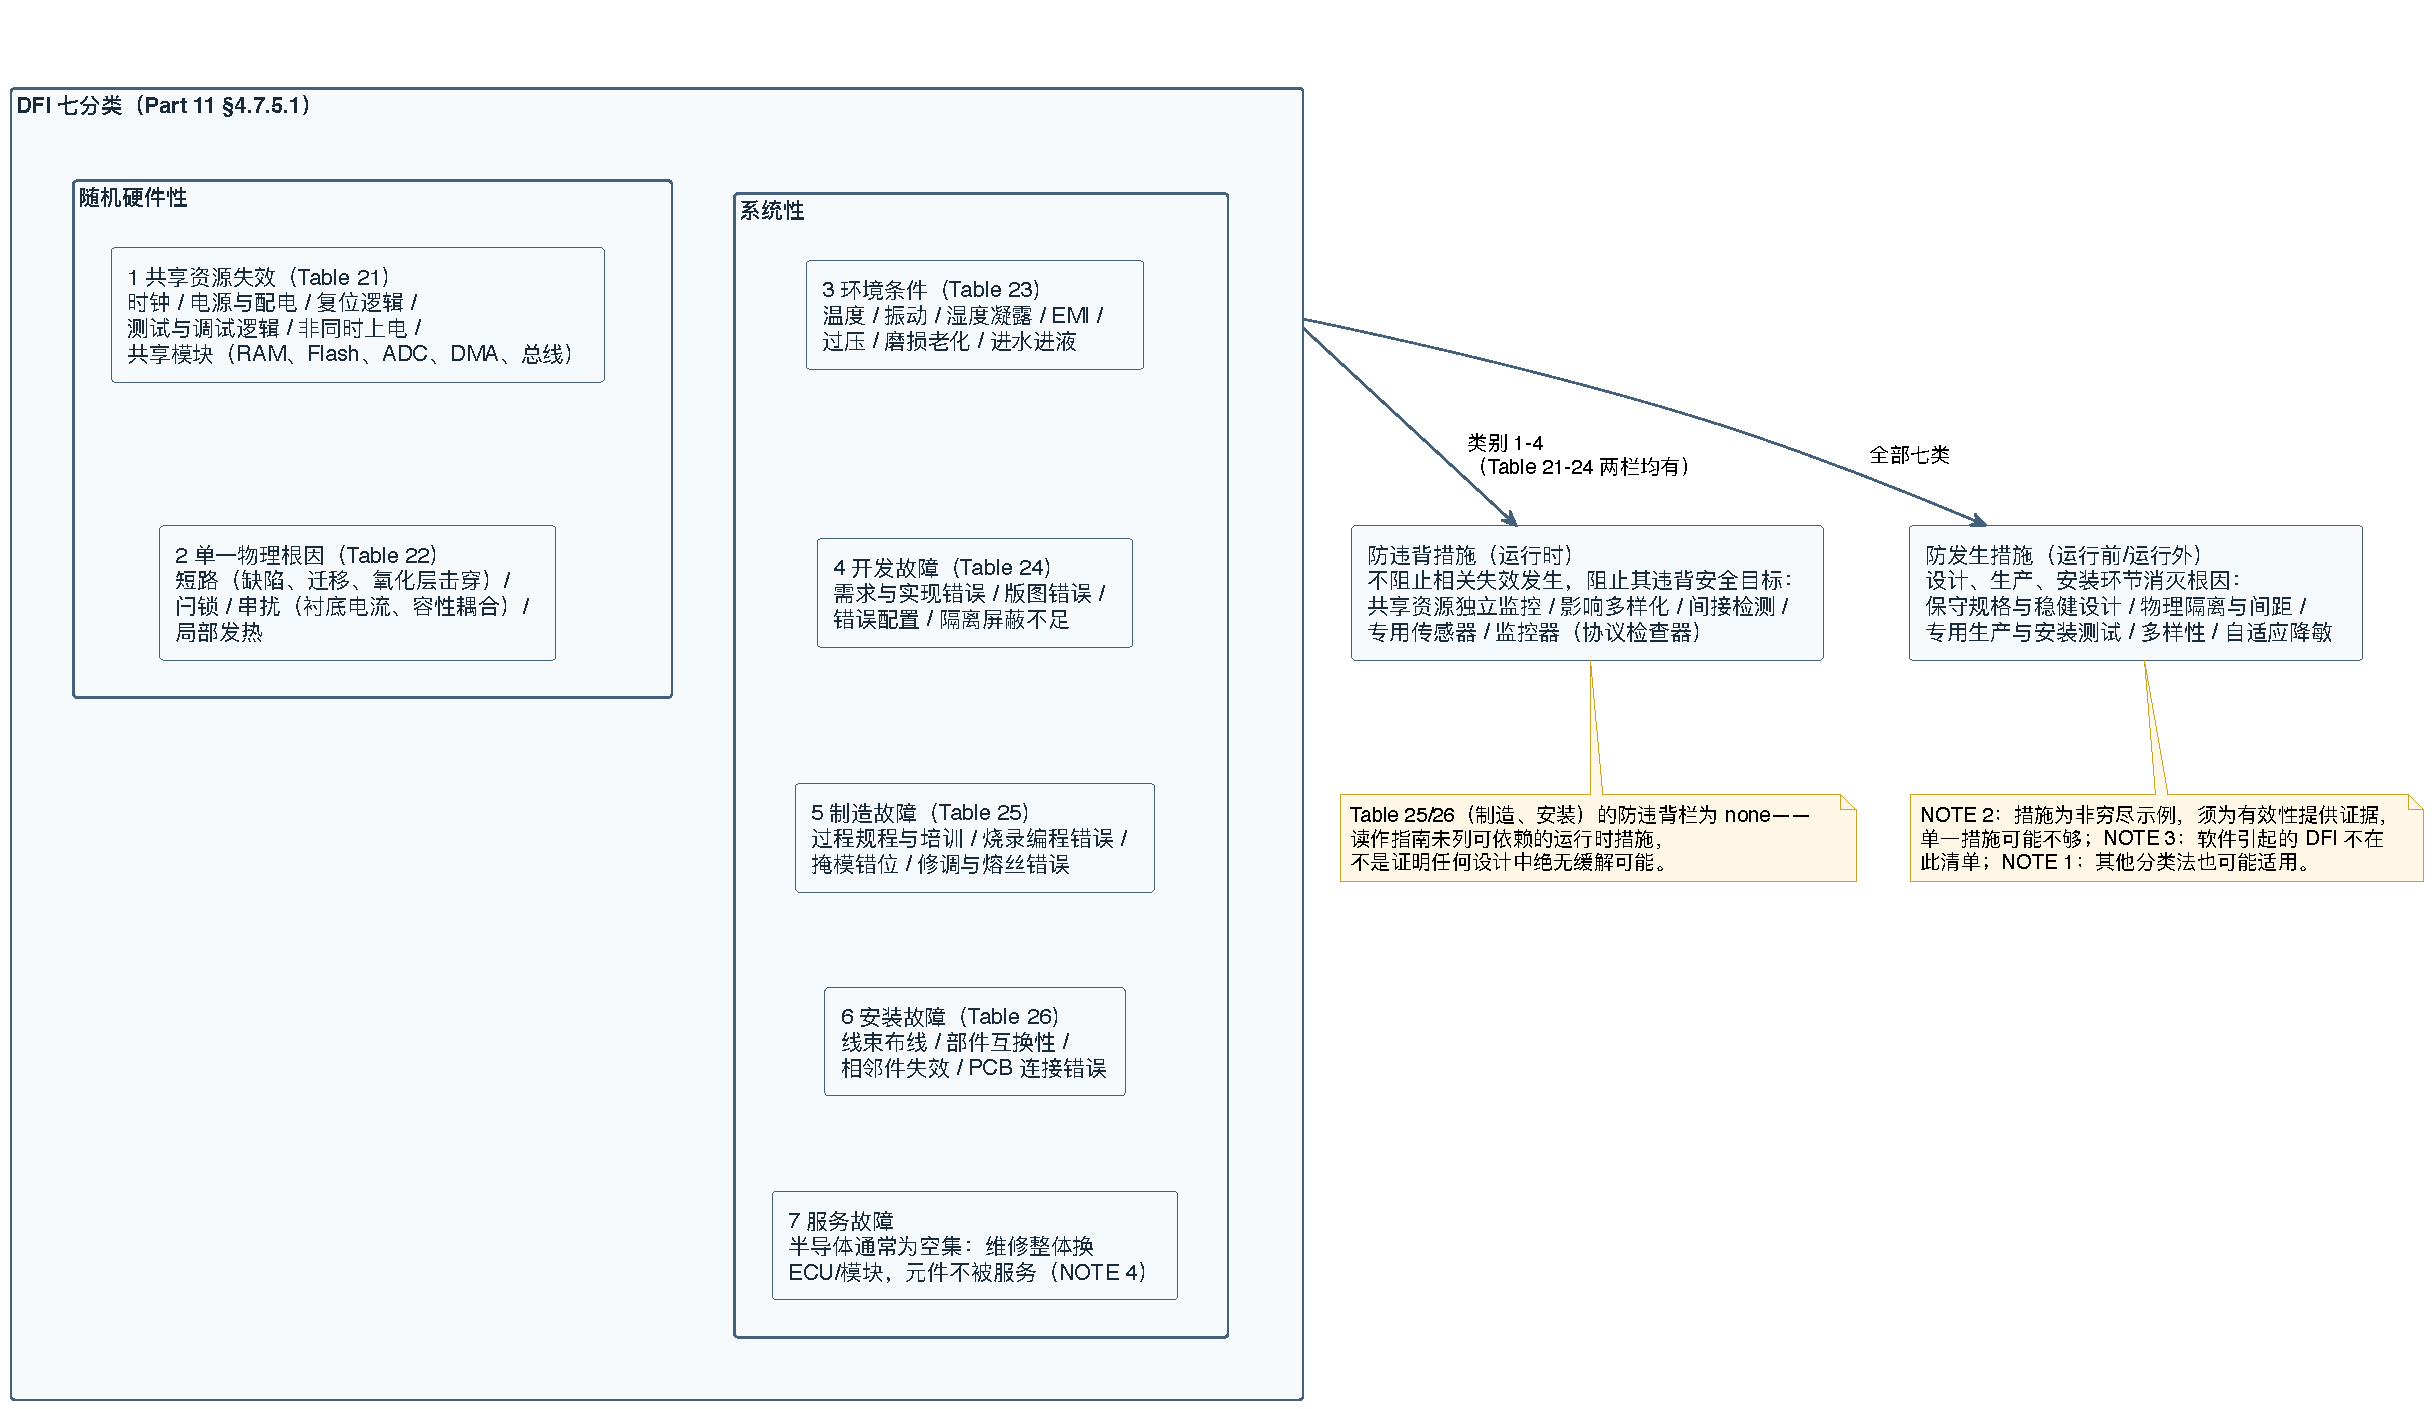
\includegraphics{figures-rendered/appA-fig3-dfi-seven-classes.pdf}}
\setcounter{figure}{2}
\caption{DFI 七分类与措施两分法——两类随机硬件性根因与五类系统性根因（服务故障对半导体通常空集），各配防违背（运行时）与防发生（运行前）两族措施；制造与安装两类在指南表中防违背栏为 none。}
\end{sidewaysfigure}

每个类别的措施分\textbf{两族}（p54）：\textbf{防违背措施}——不阻止相关失效发生，但阻止它违背安全目标（运行时检测与反应）；\textbf{防发生措施}——在运行前或运行外消灭它（设计、生产、安装环节）。这个两分法与第 6 章“覆盖率是掐断因果链，不是让元件不坏”一脉相承。把六张表压缩成一张速览（详表请回原文对应页）：

\begingroup\small
\setlength{\tabcolsep}{4pt}
\begin{xltabular}{\linewidth}{@{}XXXX@{}}
\toprule
DFI 类别 & 典型根因示例 & 防违背措施示例 & 防发生措施示例 \\
\midrule
\endhead
共享资源失效 & 时钟（PLL/时钟树/使能）、测试与调试逻辑（DFT 扫描链、调试路由、trace）、电源（配电网络/共享调节器/带隙基准）、非同时上电（闩锁/浪涌）、复位逻辑、共享模块（RAM/Flash/ADC/DMA/中断控制器/总线） & 共享资源专用独立监控（时钟监控、电压监控、存储 ECC、配置寄存器 CRC、测试/调试模式信号化）；选择性抗软错误加固；启动/运行自检；影响多样化（主查核间时钟延迟、异构主查核、不同关键路径）；间接检测（会因共享资源失效而失败的周期自检）；专用传感器（延迟线共因传感器） & 保守规格等避错措施；共享资源内部功能冗余（多过孔/触点）；故障诊断与隔离/重构；专用生产测试（能发现复杂故障的 SRAM 全检）；拆分资源以缩小共享面；自适应降敏（降压/降频） \\
单一物理根因 & 短路（局部缺陷、电/过孔/触点迁移、氧化层击穿）、闩锁、串扰（衬底电流、容性耦合）、局部发热（失效的调节器或输出驱动） & 影响多样化；间接检测或专用传感器 & 专用生产测试；物理隔离/间距设计规则；单芯片上的物理分离 \\
环境条件 & 温度、振动、压力、湿度/凝露、腐蚀、EMI、外部过压、机械应力、磨损、老化、进水进液 & 影响多样化；环境条件直接监控（温度传感器）或间接监控（延迟线） & 保守规格/稳健设计；物理分离（远离热源）；自适应降敏；限制访问频次或操作循环数（EEPROM 写次数）；封装稳健设计 \\
开发故障 & 需求/规格错误、实现错误、串扰或闩锁预防设计不足、错误配置、版图错误（冗余块上布线、绝缘/隔离/屏蔽不足）、功耗热梯度导致敏感电路失配 & 监控器（协议检查器） & 符合 ISO 26262 的设计流程；多样性（实现/功能/架构多样性或开发多样性） \\
制造故障 & 过程规程与培训问题、控制计划与特殊特性监控缺陷、烧录与产线末端编程错误（版本/条件/协议/时序）、掩模错位、末端修调或熔丝错误（激光修调、OTP/EEPROM 校准系数） & \textbf{无} & 专用生产测试；符合 ISO 26262（见 §4.9）；多样性 \\
安装故障 & 线束布线、部件互换性、相邻件失效（接口配置错误、负载错误）、PCB 连接错误、备用存储配置错误 & \textbf{无} & 专用安装测试；符合 ISO 26262；多样性 \\
\bottomrule
\end{xltabular}
\endgroup

注意 Part 11 Table 25/26 在制造与安装两类的“防违背措施”栏列为 \textbf{none}，把重点放在生产/安装前的预防与测试。应把它读成该指南没有列出可依赖的运行时措施，而不是证明所有设计中绝无任何缓解可能；具体项目仍按根因、传播路径和适用的 Part 7/9 要求分析。这为 A.6 节“在该资料性解释下全线按安全相关处理”的论证提供了一项半导体侧理由，但不证明这是唯一的生产策略。

NOTE 2 的免责声明值得带进项目模板（p54）：所列措施是\textbf{非穷尽的示例}，有效性取决于电路类型与工艺，Part 11 建议为所声称的有效性提供证据；单一措施可能不够，需组合。验证有效性的方法族见 §4.7.5.2（p58–59）：已知原理的分析法、按文档化试验协议做的\textbf{流片前仿真}（时钟/电源扰动仿真、EMI 仿真，配合故障注入产生目标扰动）、\textbf{流片后稳健性测试}（EMI、老化、加速老化、电应力）、以及有文档理由支撑的专家判断。两条边界要分层：Part 9 §7.4.2 NOTE 资料性地指出 IEC 61508 式的 \(\beta\) 因子量化\textbf{一般不是足够可靠的方法}；Part 11 则建议用\textbf{多样性}或\textbf{隔离/分离}做措施时，论证其程度与目标 DFI 相称。项目若把这两项设为放行条件，应标 \nolinkurl{BookHousePolicy}；不能称为 Part 11 shall。

\Needspace{5\baselineskip}
\subsection{B1–B12 工作流：一条有回路的流水线}

§4.7.6 用一张流程图（Figure 23，p59）把 DFA 组织成 B1–B12 十二个框，注意它不是直线而是带两处“信息不够就回炉”的回路：

\begin{itemize}
\item \textbf{B1 启动判定与元素识别}（p60）：六种情形触发 DFA——诊断功能分配到硬件/软件元素；相似或相异冗余；元件/part 上的共享资源（时钟、复位、电源、存储、ADC、I/O、测试逻辑）；共享硬件上跑多个软件任务；共享软件功能（I/O 例程、中断处理、数学库）；系统或元素级 ASIL 分解派生的独立性要求落到同一 IC 的不同元素上。输入是技术安全需求（尤其独立性/免于干扰要求）、架构描述（框图、流程图、故障树、状态图、软硬件分区）与安全措施；产出是“可能被相关失效影响的元素对/组清单”及其独立性要求。NOTE 1 顺手划了个常被忽略的边界：跑在可编程硬件上的固件与微码，无论载体叫不叫 CPU，都可视为\textbf{软件元素}（p60）。
\item \textbf{B2 DFI 识别}（p60）：以 §4.7.5.1 的典型 DFI 清单为查验表，补全架构分析没想到的已知依赖，并与定量分析中发现的依赖机制交叉核对。
\item \textbf{B3/B4 效应信息充分性判定}（p60–61）：逐个 DFI 检查现有文档是否足以判断其对目标架构的有效性；不够就补充资料、回到 B2。NOTE 推荐分层法：顶层视图看清共享资源，再下钻到“硬件 subpart+其安全措施”的分解视图找设计级依赖。
\item \textbf{B5 相关 DFI 清单固化}（p61）：经评审固化清单；随机硬件类 DFI 中\textbf{能可靠量化的部分}纳入 Part 5 Clause 8/9 的定量分析（共享振荡器输出过快时钟、调节器故障导致内部过压，见 NOTE 2 列举）；不能可靠量化的（时钟树故障的时序效应、元素与其机制间的热耦合、衬底电流）继续走定性通道。
\item \textbf{B6 措施识别}（p61）：为目标架构相关的相关失效补充必要的安全措施，§4.7.5.1 的措施列做起点，最终措施需求要文档化。
\item \textbf{B7/B8 措施信息充分性判定}（p61）：文档不足以评估措施有效性时，补充细节再回 B6。
\item \textbf{B9 措施清单固化}（p61）：经评审固化。NOTE 2 藏着一个容易漏的闭环：新增措施改变芯片面积，从而改变各部分的失效率分布——\textbf{定量分析通常要跟着更新}。
\item \textbf{B10 有效性评估}（p62）：验证方法与 Part 5 Clause 10 的安全措施验证同族——FTA/ETA/FMEA、故障注入仿真、基于工艺资格测试的设计规则、电压等级或间距的过设计、温度/过压应力测试、EMC 与 ESD 测试、专家判断。两条 NOTE：实现措施的元素本身也要计入 Clause 8/9 的定量分析；\textbf{新引入的措施自己也可能成为相关失效的宿主}，此时对新依赖重新走一遍 DFA 程序。
\item \textbf{B11/B12 风险充分性评估与措施改进}（p62）：评估剩余风险；不充分则改进措施（B12）并重评。可量化的残余风险计入定量分析——例如功能与其安全机制被同一相关失效波及时，把机制的失效模式覆盖率\textbf{按未缓解的依赖折减}。结尾的 NOTE 把定量与定性的分工再说了一遍：若定量度量目标已达成，随机硬件视角的风险即视为足够低，即使受影响元素没有专门措施；同一元素上的系统性 DFI 仍在 DFA 里定性处理，并可能独立于定量结果引出措施。
\end{itemize}

硬件与软件之间的相关失效通常分开考虑，只有当“针对硬件的安全机制用软件实现”时才合并分析（§4.7.8，p63）。两个原文例子：软件 CPU 自检与独立硬件看门狗互为兜底——CPU 坏了，自检抓不到就由看门狗抓；E-GAS 三层监控概念中 L2 软件监控 L1 软件，两层本身相异，为进一步压低硬件相关失效导致安全目标违背的概率，再加程序流监控、CPU 自检、L2 关键变量在 RAM 中反码冗余存储、独立的质询-应答看门狗。

Annex B（p144–157）给了两个完整判例，值得多花一段拆它的论证结构。\textbf{微控制器例}（B.1，p144–148）：分析对象是一颗带冗余 CPU 的微控制器，安全需求被刻意精简到两条便于聚焦——MCU-REQ-1 要求“硬件元素 1.1 处理信号 1 的故障须在 20 ms 内检出”，其子需求规定由硬件元素 1.2 冗余处理、软件比对结果、不一致时经看门狗接口报错；MCU-REQ-2 要求“导致 CPU 错误输出的随机硬件故障须在 20 ms 内检出”，子需求规定冗余 CPU 逐拍硬件比对、不一致即产生错误事件（p146）。这些都是 Annex B 判例内部的需求，不是可复用到其他 MCU 的 20 ms 标准值。DFA 只聚焦有潜力违背 MCU-REQ-2 的 DFI，沿工作流走：B1/B2 阶段用一棵\textbf{定性故障树}（Figure B.2）分析架构，把共享资源（时钟、电源、复位）与冗余元素摆上台面；然后逐行落进一张五列账表（Table B.1，p147）：元素—冗余元素—DFI（分“共享资源”与“单一物理根因”两列）—故障的避免(A)或控制(C)措施—验证方法。表中每条措施都标了 A/C 属性（对应 §4.7.5.1 的两分法），并留出验证方法列。本书由此采用一条 \nolinkurl{BookHousePolicy}：未给出有效性验证方法的措施仍是候选措施，不标记为已闭环。\textbf{模拟例}（B.2，p149–157）走查两类场景：共享电压调节器（B.2.2）与耦合机制（B.2.3，衬底耦合、热耦合这类“看不见的线”），示范了当 DFI 无法量化时定性论证怎么写。判例的正确用法与第 4 章 HARA 判例目录相同：\textbf{学它的论证结构，不复制它的结论}——你的芯片的共享资源清单、措施与覆盖率，都要从你自己的架构分析里长出来。

最后是本书的状态纪律（\nolinkurl{BookHousePolicy}，回指第 8 章的放行语义）：把 B1–B12 建成流程模型、把七类 DFI 建成分类表，都只是\textbf{结构就绪}；每一条具体依赖的可信度判定、措施有效性证据、评审结论必须落在各自状态词表，不能由流程图存在推断完成。\textbf{工作流画完不等于 DFA 做完，DFA 做完不等于独立性成立}——中间隔着证据。

\Needspace{6\baselineskip}
\section{故障注入与验证证据}

\Needspace{5\baselineskip}
\subsection{故障注入能回答什么问题}

故障注入——人为把故障塞进设计或实物、观察安全机制接不接得住——在附录 D 的集成测试与软件测试方法表里都露过面。Part 11 §4.8 讲它在半导体层的专门用法（p63）：支撑硬件架构度量的评估；评估安全机制的诊断覆盖率（软件自检、硬件内建自检）；评估诊断时间间隔与故障反应时间间隔——回指第 2 章的时间间隔家族；确认故障效应（例如计算瞬态故障的架构脆弱性因子：一个故障在特定输入下产生可观察错误的概率）；以及支撑安全机制的流片前验证（触发机制、验证软件级反应、验证边角用例、验证互连）。

规模问题有官方台阶（NOTE 1，p63）：若以合理资源在合理时间内做不完精确注入，可以缩小战役范围（只在 IP 块级注入）、只用分析法、或分析与注入组合。台阶不是滑梯——缩了范围，结论的适用范围也要跟着缩。

\Needspace{5\baselineskip}
\subsection{把一次注入战役写成一个实验对象}

§4.8.2（p63–65）资料性地给出一份可帮助验证策划、并建议在策划中描述和论证的信息清单。本书把它操作化为\textbf{七元组实验对象}——目标、故障模型、注入位置、注入时间、观测量、判定准则、结果。七元组是 \nolinkurl{BookHousePolicy}，不是 Part 11 原生数据模型。逐项拆开：

\begin{itemize}
\item \textbf{故障模型与抽象层级}：stuck-at 注在门级网表，位翻转在 RTL 级就够（EXAMPLE 1）；层级选择还取决于所需精度——用门级网表对 CPU 软件自检做端口/网络故障注入，置信度高（EXAMPLE 2）。Part 11 建议给出层级选择理由；本书将其设为接收条件。
\item \textbf{观测点与诊断点}：在哪一层看故障效应（观测点）、在哪一层看机制反应（诊断点）。奇偶校验电路的覆盖率验证可设在 part/subpart 级；跨 IO 回环验证设在顶层（EXAMPLE 3/4）。顶层注入不可行时，Part 11 给出用\textbf{功能等价模型}替代安全机制的资料性做法（例如把看门狗换成等价模型），并建议提供“模型充分反映机制安全特性”的证据（NOTE 3、EXAMPLE 5）；本书将这份证据设为接收条件。
\item \textbf{注入方法}：已知故障位置的直接注入、形式化方法注入、仿真加速器（emulation）注入、辐照注入（EXAMPLE 6）。
\item \textbf{故障位置与故障清单}：与被验证的失效模式挂钩。Part 11 允许在有理由时抽样，并在 NOTE 5 列出样本量 n、样本分析结果 p（如机制检出 stuck-at 的比例）、期望置信度、误差边界与统计独立性；原文用 \(\alpha\) 表示“desired confidence”，统计计划应明确 \(\alpha\) 究竟指置信水平还是通常意义上的显著性水平。也可用故障折叠（fault collapsing）把故障群压缩到质故障。范围裁剪要有机理依据：验证双核锁步的覆盖率，相关故障群可以限于被比较的 CPU 输出及相关位置；验证软件自检，相关的是 CPU 内部故障（EXAMPLE 7/8）。本书要求预先冻结这些选择，规则依据为 \nolinkurl{BookHousePolicy}。
\item \textbf{注入控制}：注什么类型、瞬态持续多久、一次仿真注几个、何时何地注、观察窗开多大（EXAMPLE 9）。
\end{itemize}

抽样的统计学值得停一拍做算术直觉（教学示例，非 Part 11 原文数值）。假设某安全机制的目标覆盖率主张是 99\%，从百万级故障空间抽取 n = 1 000 个故障，机制检出 995 个，点估计 \(\hat{p}\) = 99.5\%。用预先选定的\textbf{双侧 95\% Wilson score 区间}计算，区间约为 \textbf{[98.835\%, 99.786\%]}；下界低于 99\%，所以这批数据不能按该判据背书“覆盖率至少 99\%”。若只抽 n = 100 并检出 99 个，Wilson 95\% 区间更宽，约为 \textbf{[94.551\%, 99.823\%]}。若验收问题只关心下界，可预先规定单侧下置信限与构造方法，但不能看到结果后再换口径；即使用单侧 95\% Wilson 下限，995/1 000 也只有约 \textbf{98.976\%}，仍低于 99\%。

这里的“95\%”也不是“真实覆盖率有 95\% 概率落在本次区间内”：在频率学解释中，真实覆盖率是固定参数；若反复采用同一抽样机制和 Wilson 构造方法，长期约 95\% 的区间会覆盖它。这个解释还依赖二项模型、代表性抽样与独立性；故障折叠、分层抽样或相关注入会改变有效样本量，不能把公式机械套上。Part 11 NOTE 5 只是资料性地列出 n、p、置信度、区间与统计独立性；本书要求预注册统计方案并以区间下界放行，属于 \nolinkurl{BookHousePolicy}。
\begin{itemize}
\item \textbf{工作负载}：验证锁步比较器的完整性，基础负载即可（只需激励 CPU 输出）；验证非对称冗余的覆盖率，用功能测试集派生的激励；验证瞬态故障的安全故障占比，用接近实际用例的负载；验证软件自检——\textbf{负载主要就是自检程序本身}（EXAMPLE 10–13）。不同负载会激活不同故障与传播路径，选择不匹配可能使覆盖率产生方向性偏差；因而负载是需要单列理由的偏差源，不应用“最隐蔽”这类无数据排名代替论证。
\end{itemize}

\Needspace{5\baselineskip}
\subsection{结果的用途与两条诚实条款}

注入结果可用于验证安全概念与其底层假设：机制有效性、诊断覆盖率、安全故障数量（§4.8.3，p65）。两条 NOTE 都是资料性证据指南：NOTE 1 建议为功能安全审核保留注入证据；NOTE 2 说明仿真的故障与安全分析里识别的故障\textbf{不总是一一对应}（例如开路故障难以直接仿真），可用其他代表性故障的结果精化分析（如 5.1.10.2 的 N-detect 法），同时为替代关系提供理由。本书进一步要求“做过注入”必须对应可复核的七元组战役记录；这是 \nolinkurl{BookHousePolicy}，不是 NOTE 被提升成了 shall。

把七元组落成一张随身检查单（本表为本书归纳）：

\begin{center}
\begingroup\small
\setlength{\tabcolsep}{4pt}
\begin{tabularx}{\linewidth}{@{}XXX@{}}
\toprule
元组项 & 要写清的问题 & 常见缺口 \\
\midrule
目标 & 这次战役支撑哪条覆盖率/时间量主张 & 一次注入背书多条主张，范围含混 \\
故障模型+抽象层 & 注的是什么故障、在哪一层注、为何该层足够 & RTL 层注 stuck-at 却主张门级覆盖 \\
注入位置+清单 & 故障群怎么选的、抽样统计要素齐不齐 & 只报点估计 p，不报 n 与置信区间 \\
注入时间/控制 & 何时注、持续多久、观察窗多大 & 观察窗短于故障反应时间 \\
观测点/诊断点 & 在哪看效应、在哪看机制反应 & 用等价模型替代机制却无充分性证据 \\
判定准则 & 什么算检出、什么算安全故障 & “无输出差异”与“机制报警”混判 \\
结果工件 & 记录存在哪、审计时拿什么复现 & 只留结论表，不留战役配置 \\
\bottomrule
\end{tabularx}
\endgroup
\end{center}

对仗收口：\textbf{注入回答的是“机制接得住吗”，七元组回答的是“你凭什么这么说”}。把七元组对象化成知识模型，是 A.8 节的练习题之一。

\Needspace{6\baselineskip}
\section{生产、分布式开发与确认接口}

\Needspace{5\baselineskip}
\subsection{生产：标准流程、全线安全相关}

第 9 章讲过 Part 7 的两大目标：开发并维持安全相关产品的生产过程。落到半导体（§4.9.1，p65–66），Part 11 给出两个行业解释。其一，半导体用的是\textbf{标准化生产流程}——晶圆加工、装配各工序（扩散、氧化沉积、离子注入、贴装）为特定产品单独开流程的情况很少；其二，指南认为通常无法把流程步骤清楚分成安全相关与非安全相关，因此在该解释下\textbf{全部按安全相关处理}。风险缓解可复用过程 FMEA 与控制计划等质量工具：制造测试对照电气规格验证产品、过程控制规格对照控制计划验证过程，两头合起来支撑“制造出的元件符合含硬件安全需求在内的要求”。“全线按安全相关处理”是 Part 11 的资料性解释；具体生产义务仍来自适用的 Part 7 Clause 5/6。

Part 11 §4.9.2 资料性地说明工作产物可复用（p66）：满足 IATF 16949 的质量管理体系文档可能部分或全部支撑 Part 7 Clause 5/6——生产控制计划的安全相关内容可复用质量体系控制计划，控制措施报告同理。\textbf{复用的是证据，不是自动合规或豁免}：是否满足要求仍回到 Part 7 逐项判断。这里与 A.4.3 的 DFI 速览表首尾呼应：制造类 DFI 的“防违背措施”一栏列为 \nolinkurl{none}，提醒读者不要把运行时措施当作一定存在的后手；但这一表项本身不证明掩模错位、末端修调错误在所有设计中都绝无运行时缓解。本书的工程归纳是：对这类根因，生产预防与检出通常是主要防线，这也是“在该解释下全线安全相关”的工程理由之一。

Part 11 §4.9.3 资料性地观察到：半导体元件通常不单独维护或维修，相关服务/退役活动往往可在安全计划中裁剪，供需双方也可在 DIA 中对齐预期（p66）。实际裁剪须按 Part 2 §6.4.5 给出上下文理由，不能仅凭 Part 11 的通常情形自动省略工作产物。

\Needspace{5\baselineskip}
\subsection{分布式开发：一颗芯片的上下游}

§4.10（p66–67）资料性地说明半导体开发者常具有双重角色：向 Tier 1 或半导体集成方供货时，它可处于 Part 8 Clause 5 的\textbf{供应商}角色；采购 IP、封测服务时又处于\textbf{客户}角色。DIA、供应商安全计划、供应商选择等具体义务须按 Part 8 Clause 5 的适用条件判定，不能从 Part 11 的角色示例直接推出。指南还把安全相关分布式开发的最低层级解释为安全责任终止的层级；再往下的供应商（如生产材料供应商）可由质量管理体系等其他要求约束。它与第 10 章 DIA 的 a)–k) 条目框架兼容，补充的是“同一主体在链条中双重角色”的半导体常态。

\Needspace{5\baselineskip}
\subsection{确认措施与集成验证的半导体裁剪}

确认措施——第 3 章首讲的确认评审、功能安全审核与功能安全评估——在半导体开发中需按上下文裁剪。Part 11 §4.11 资料性地给出 SEooC/IP 场景的裁剪示例，并指出相关项层面的确认评审通常超出半导体供应商范围（p67）；实际裁剪仍须按 Part 2 §6.4.5 等适用条款给出理由。指南还示例用\textbf{过程安全审核}（Process Safety Audit, PSA）落地审核；一旦选定某项 Part 2 Table 1 确认措施，其独立性等级仍由该规范表决定——资料性示例不能降低等级。

硬件集成与验证的对接见 §4.12（p67–68）：Table 27/28 逐行解释 Part 5 Table 10/11 的方法在半导体层怎么读——“需求分析”对应流片前（仿真级）与流片后（硅片级）验证；“内外接口分析”对应 IC 集成与 IO 相关的验证活动；“共因限制条件分析”对应时钟/电源/温度/EMI 测试；“环境与使用条件分析”对应温度循环、软错误率实验、高温工作寿命测试；“标准”对应 CAN/I2C/UART/SPI 等协议标准；“显著变体分析”对应工艺偏差/电压/温度（PVT）特性化测试。Part 11 把表格称为“起点”并建议按用例修改时给出理由（NOTE 1）；方法的规范性推荐度仍须回到 Part 5 Table 10/11。还有一处术语校准（p68）：“test case”在系统与半导体两界含义不同：流片后验证针对少量样品、聚焦正确集成与系统性故障；\textbf{量产测试}针对全部器件、聚焦生产引入的故障，采用结构化测试——后者属于“生产”语境，不等同于硬件集成验证。等价类与错误猜测两法在半导体测试中通常不太适用（p68）。

\Needspace{6\baselineskip}
\section{五类技术案例：同一问题框走五遍}

Part 11 §5（p68–140）按技术类型给了五份“应用说明”。本节用同一个问题框走五遍：\textbf{这类技术的故障模型是什么？安全机制改变了什么？定量分析需要哪些假设？还有哪些系统性故障需要人类审查？}每小节末尾给出安全文档（安全手册）的落点。用同一个框有两个目的：一是让你在换技术领域时带着熟悉的问题清单上手，而不是从零学一遍“这个领域的规矩”；二是暴露各领域真正的差异所在——问题相同、答案不同的地方，才是该领域的知识增量。

\Needspace{5\baselineskip}
\subsection{数字元件与存储器（§5.1，p68–88）}

\textbf{故障模型}。非存储数字逻辑的永久故障：stuck-at（节点恒 0/恒 1）、开路（节点或互连断裂）、桥接（相邻信号意外连通，因电路结构呈线或/线与）、单粒子硬错误 SHE（单次辐射事件造成永久损伤，如栅氧破裂）；瞬态故障：单粒子瞬态 SET（节点上的瞬时电压尖峰）、单粒子翻转 SEU、单比特翻转 SBU、多单元翻转 MCU（一次事件翻多个通常物理相邻的位）、多比特翻转 MBU（同一字节/字内多位错——简单单纠 ECC 纠不了）（§5.1.2，p68–69）。NOTE 3 给出“等效覆盖”论证思路：针对 stuck-at 设计的机制可在有对应性理由时声称覆盖最终表现为 stuck-at 的桥接/开路故障。存储器故障模型另有一表（Table 29，p70）：Flash/ROM/OTP/eFUSE/EEPROM/RAM/DRAM 各配 stuck-at 加一族附加模型（stuck-open、耦合故障、寻址故障、过渡故障、邻域图形敏感故障、擦写扰动等）。Part 11 NOTE 1 说明，典型应力条件通常只能激活其中一部分，其他模型可在产线末端测试设备上激活，并要求用证据说明测试对应条件下的有效性；本书把该说明设为覆盖率主张的接收条件。

\textbf{失效模式的定义术}。§5.1.4（p70）给出四缺省键：功能缺失（FM1，该给不给）、功能误动（FM2，不该给却给）、时序错误（FM3，给早给晚）、数值错误（FM4，给错内容）。好的失效模式集有三判据：能把工艺故障映上来、能支撑诊断覆盖率评估、理想情况下各模式不相交。Table 30（p71–74）按此框架给出 CPU、中断处理、MMU、中断控制器、DMA、总线、SDRAM 控制器（并演示第二层抽象：行地址/列地址/命令/数据通道分列）、外部与嵌入式 Flash、SRAM、数据一致性、通信外设（CAN/FlexRay/以太网/SPI）、信号处理加速器的示范定义——FMEDA 排到哪个模块，先来这张表对号。

\textbf{定量分析的假设}。永久故障：分层划分（工具可辅助检查跨模块边界的一致性与完整性，但不能单独保证语义无遗漏）\(\rightarrow\)按面积或按门数摊失效率（CPU 占裸片 3\% 面积即摊 3\% 失效率）\(\rightarrow\)分类为安全/残余/检出双点/潜伏双点故障\(\rightarrow\)定失效模式覆盖率（可把寄存器组拆到单个寄存器逐个算再合并）（§5.1.7.1，p75–77）。瞬态故障单独立账（§5.1.7.2，p77）：RAM 密度高，瞬态失效率常显著高于逻辑，Part 5 §8.4.7 NOTE 1 建议为 RAM 与其余部分\textbf{分开算度量}；安全故障占比是瞬态分析的主角——原文例子值得手算：一个每 10 ms 写一次、写后 1 ms 用一次的寄存器，瞬态故障只有落在那 1 ms 窗口内才可能违背安全目标，其余 9 ms 都是安全故障，安全占比 90\%。瞬态不算潜伏故障覆盖——根因转瞬即逝，错误状态大概率在下一个下电周期被清除（NOTE 2）。\textbf{需特别核对的限定}：Part 5 Annex D 的覆盖率表部分数值\textbf{只对永久故障有效}——RAM March 测试对永久故障覆盖“高”，对软错误覆盖为\textbf{零}（§5.1.7.2.2 EXAMPLE 2，p77）；因此引用 Annex D 数值时要同时标明故障类型与适用条件。

\textbf{安全机制清单}（§5.1.13，p85–88）：存储 ECC（检纠能力随冗余位数）、修正校验和、存储签名、块复制（双存储硬件或软件比对）、RAM 图形测试、奇偶位、RAM March 测试（通常只能在初始化或停机时运行，NOTE 2）、运行校验和/CRC（漏检概率 1/2\^{}n，n 为校验和位数；随存储增大覆盖率下降）。每条机制在原文都有“目标—描述—适用限制”三段，选型时连限制一起抄。

\textbf{系统性故障与文档}。§5.1.9 把 RTL 设计阶段的避错技术与 Part 5 表格挂接（p78–82），供数字 IP 的开发过程审查用；黑盒软 IP 的集成者还可参照 Part 6 相应表格类比处理编译产物（§4.5.5 NOTE 3，p23）。安全文档形态见 §5.1.11（p83）。

\textbf{判例走查：DMA 的覆盖率是怎么估出来的}（Annex A，p140–143）。这是 Part 11 里最适合手算的一个完整判例，把“失效模式定义\(\rightarrow\)机制映射\(\rightarrow\)覆盖率估算”三步走通。用例设定：通信外设每 X ms 收一条消息，触发 DMA 请求；DMA 把消息从外设接收缓冲搬到固定 RAM 区，完成后触发 CPU 中断；CPU 再按消息 ID 把消息拷到另一块 DMA 无权访问的 RAM 区。四个安全机制站好位：专用存储保护单元（限制 DMA 只能写目的地址、读源地址）、端到端保护（8 位 CRC + 4 位消息 ID + 4 位消息计数器，16 个 ID 里只有 12 个合法）、超时监控、中断源合法性监控。

然后按 Table 30 的四键失效模式逐个对号。\textbf{DMA\_FM1（该传不传）}：超时监控在时限内等不到传输完成信号，判例覆盖率估 100\%。\textbf{DMA\_FM2（不该传却传）}拆成两个子模式，覆盖率的估法完全不同——DMA\_FM2.1 搬的是\textbf{上一条}消息：内容合法但计数器/ID 对不上，端到端保护抓个正着，判例估 100\%；DMA\_FM2.2 搬的是\textbf{随机值}（按“白噪声”建模，每个错误状态等概率）：只有当随机数据同时碰对合法 CRC、合法 ID、正确计数器，错误才会漏网。三个概率相乘：p = (1/2\(^{8}\)) \(\times\) (12/16) \(\times\) (1/2\(^{4}\)) = (1/256) \(\times\) 0.75 \(\times\) (1/16) \(\approx\) 0.000 183，覆盖率 = 1 - p \(\approx\) \textbf{99.98\%}（p141；数值两源核对一致）。手算复核：0.75/4096 = 1.831\(\times\)10\(^{-4}\) \checkmark{}。\textbf{DMA\_FM3（时序错）}的子模式里，“取数期间被下一条消息部分覆盖”的最坏情形假设 ID 必然合法（p=1）、计数器最坏也合法（p=1），只剩 CRC 一道网：覆盖率 = 1 - 1/2\(^{8}\) \(\approx\) \textbf{99.6\%}（p142）——保守估算取两个子模式中较低者。\textbf{DMA\_FM4（值错）}再细分：读写方向颠倒由端到端保护和存储保护单元检出，判例估 100\%；访问宽度错按端到端校验估 99.6\%；访问地址错由存储保护单元检出，估 100\%；数据输出错按白噪声归到 99.98\%；错误中断请求在该用例的单一中断源假设下由中断源监控检出，估 100\%（p143）。这些 100\%/99.98\%/99.6\% 均是 Annex A 特定架构、失效模式细分与概率假设下的估计，不是元件认证值，也不能直接迁移到其他设计。

这个判例教的不是那几个百分数，而是三条方法论：\textbf{覆盖率是逐失效模式、逐机制组合估出来的}，不存在“这个模块覆盖率 99\%”的整体拍板；本书的接收策略是\textbf{只在明确写出随机模型时接受概率论证}（白噪声假设要写明），确定性检测（超时、地址保护）直接给 100\% 时也注明机理；\textbf{子模式分布未知时取保守下界}。更精确的总覆盖率还要乘上 FM2.1/FM2.2 之间的失效分布——分布不知道，可参照 §4.3.3 的均匀假设并做敏感性分析。这三条是从 Part 11 判例提炼的 \nolinkurl{BookHousePolicy}，不是判例自身产生的 shall。

\Needspace{5\baselineskip}
\subsection{模拟与混合信号元件（§5.2，p88–109）}

\textbf{划分}。信号不限于数字状态的元素即模拟元素；混合信号元件至少含一个模拟与一个数字元素，建议明确分界，因为两者的设计、版图、验证、测试方法论与工具可能存在显著差异（§5.2.1，p88）。切分子元素的判据：信号流（反馈 ADC—数字调节器—输出驱动构成的控制环）、连通性（基准与偏置电路服务多个模拟块）、工艺差异（HV 开关是 DMOS，栅驱动是常规 MOS——失效率可能差数量级、故障模型也不同）、电源域差异、频率分区（p89）。一条反内卷提示：\textbf{粒度更细未必让安全分析更好}——细到超过安全需求、安全机制与独立性证据的需要，只是徒增工作量（p89）。

\textbf{失效模式是语境的函数}。这是模拟节最重要的一课（§5.2.2.1，p90）。同一个电压调节器：常识失效模式是过压/欠压，配 OV/UV 监控即可；但当它作为\textbf{传感器供电或 ADC 基准}，阈值之内的精度漂移与振荡同样致命——要靠独立 ADC 周期回测；当它给\textbf{射频模块}供电，纹波抑制比（PSRR）成了安全属性——阈值内的纹波与尖峰要低通滤波兜底；当它给 MCU 内核供电且启动过快导致浪涌压降，软启动功能就是缓解措施。四个例子同一器件、四种失效模式清单——\textbf{先问“它在系统里当什么”，再开失效模式清单}。把失效模式判为非安全相关时要在安全分析中留理由；失效模式分布由半导体供应商给出定量数据，且各模式分布之和按 100\% 处理（NOTE 2）——这是定量分析能做加法的前提。Table 36（p91–98）给出各类模拟 part/subpart 的失效模式参考清单，可用来扩充 Part 5 Annex D。瞬态方面（§5.2.2.2，p98）模拟电路对软错误相对钝感，但混合信号里的数字辅助逻辑照旧要考虑。

\textbf{粒度的两难有原文判例}（§5.2.3.2，p99）。一个线性稳压器配窗式电压监控（1.2 V \(\pm\) 0.12 V 之外算故障）：分析停在稳压器\textbf{输出端}，容易区分安全/危险失效并量化监控的保护效果，但难以量化每类失效的可能性；分析下钻到内部\textbf{带隙基准}，传播路径与可能性好分析了，监控对带隙本身的保护又难量化了。取舍规则：安全机制在系统/元素级时，往下钻只会徒增复杂度；要量化失效分布时，适度下钻反而更准——对稳压器五个失效模式做均匀分布，不如对带隙、缓冲、驱动这些 subpart 做均匀分布再合并（按 §4.2 术语：稳压器是 part，带隙/缓冲/驱动是 subpart）。分布来源两档（§5.2.3.3，p99–100）：初始分析用均匀分布（五个模式各 20\%），细化时按根因电路的面积占比给。

\textbf{模拟元件的安全故障有天然来源}（§5.2.3.4，p100）。模拟信号是连续的，分配给模拟元件的安全需求容差往往比元件自身实际容差\textbf{松}——参数漂移落在需求容差之内的那部分失效就是安全故障。三个原文例子：限流电阻阻值漂移 50\% 但仍能限流，安全；输出驱动的摆率控制只为 EMI 服务、与安全目标无关，其失效安全；稳压器只给数字电路供电时，阈值内的精度与稳定性失效安全——与本小节开头“给 ADC 做基准”的场景对照：\textbf{同一失效模式，换个下游就换一次分类}。

\textbf{安全机制}（§5.2.4，p102–105）：上拉/下拉电阻、过压/欠压监控、电压钳位、过流监控、限流、上电复位、模拟看门狗、滤波器、热监控、模拟内建自检、ADC 监控、ADC 衰减检测、ADC 通道卡死检测。\textbf{定量核查}：架构度量计算的验证单列一节（§5.2.3.7，p101）；混合信号的软错误只在数字部分按 5.1.7.2 处理——模拟电路的辐照软错误率测量困难，主要靠更细的分析替代（p99 NOTE）。\textbf{系统性故障}：开发阶段避错技术表（§5.2.5，p105–108）覆盖稳健设计、原理图检查等人工与工具手段。安全文档：与数字侧同构的“安全手册/安全应用笔记”，外加失效率计算信息（如晶体管数）与 AoU 描述（§5.2.6，p108–109）。

\Needspace{5\baselineskip}
\subsection{可编程逻辑器件（§5.3，p109–124）}

\textbf{对象}。PLD = 可配置 I/O + 非固定功能（逻辑块+用户存储+配置技术）+ 布线资源 + 固定功能（时钟/电源/复位，复杂器件还有硬核 CPU、存储控制器）（§5.3.1.1，p109–110）。类型从一次可编程的 PAL、可重编程的 GAL、非易失的 CPLD 到以易失 SRAM 配置为主的 FPGA（Table 42，p111）。配置技术是安全链的正式一环——易失与非易失工艺的安全能力不同（NOTE，p110）。

\textbf{生命周期的双主体裁剪}。PLD 的特殊性在于\textbf{制造者与使用者分担生命周期}（§5.3.1.3，p111–113）：PLD 制造者负责器件本身，PLD 用户在器件上实现自己的电路。Part 11 逐部给出适用性解释：Part 2 的活动可按双方贡献裁剪，相关项级 HARA 等活动通常不落在仅作为器件供应商的制造者；Part 3 通常不适用于制造者，除非其兼任相关项集成角色；Part 4 可在 SEooC 场景按上下文应用；Part 5 的相关活动由双方按各自贡献考虑；Part 6 主要涉及高层次综合流程（OpenCL、C 转 HDL、基于模型），传统 HDL 流程更多回到 Part 5；Part 7 对应配置烧录的生产控制。无内建机制时，指南建议制造者提供基础失效率、失效模式与分布，特定设计的度量由掌握实现上下文的用户计算；Table 52 又把配置正确性检查（如校验和）列为集成验证方法。以上是 Part 11 的裁剪指南；实际项目仍需按适用性逐项回到相关 Parts 的条款，不能把“Part 5 全部条款对双方适用”当成未经裁剪的总括 shall。

\textbf{故障模型与失效模式}。PLD 的失效模式表（Table 43，p114）按 Figure 25 的结构分块给：固定功能 IP 与数字/模拟 I/O 直接回指数字节的 Table 30、Part 5 Table D.1 与模拟节的 Table 36——固定功能通常独立成区，可参照普通数字/模拟元件的相应方法处理；\textbf{逻辑块}的失效模式是“所实现功能的永久/瞬态损坏”；\textbf{配置技术}的失效模式是“逻辑块配置被永久/瞬态意外改变”——瞬态项的相关性取决于 PLD 工艺。SRAM 配置器件与 Flash/反熔丝等非易失工艺的安全能力可能不同；反熔丝工艺是否对某类瞬态故障不敏感，仍须按具体器件工艺与供应商证据判断。\textbf{布线资源}的失效模式是“一组逻辑块共同实现的功能损坏（含时延变化）”，配置技术自身的连线也归入布线资源。这张表示范了一个建模要点：\textbf{同一物理故障（配置位翻转）在 PLD 里被拆成“功能损坏”与“配置改变”两个语义层}，因为两者的检测机制不同——前者靠功能级冗余或自检，后者靠配置校验和/回读。

\textbf{定量与 DFA}。PLD 裸片失效率可按 §4.6.2.1.1 的模型算，配置技术的晶体管既可单列一项、也可摊进逻辑块与用户存储（§5.3.3.1.1，p114–116）；瞬态失效率示例见 §5.3.3.1.2。失效模式分布的三种算法（Table 47，p118）值得对照：a) 均匀分布（四个失效模式各 25\%）；b) 按各失效模式牵涉子部件\textbf{估计}消耗的逻辑块数加权（10/110 = 9.09\% 起）；c) 按\textbf{实测}的资源贡献计算（细到“总线接口对两个数据类失效模式各贡献 50\%、对配置失效模式贡献 100\%”）——精度逐级上升，工作量也是。用户侧故障注入有个现实困难：不知道自己的设计被映射到哪些逻辑块。§5.3.3.1.4 的出路是在映射前的逻辑设计上注入（例如把用户 RTL 综合成参考网表再注入），但要论证“注入的故障相对假定实现是有意义的”（p118）。DFA 按 §4.7 的流程走，Table 48（p119）逐步列出制造者与用户各自的特殊性——布线资源与配置存储是 PLD 特有的共享资源。安全机制示例（§5.3.4，p120）与系统性避错（§5.3.5，p121–123）分制造者侧（工艺、基础架构）与用户侧（设计流程、支撑工具——工具置信度回指第 10 章 TCL 框架）。生产侧同样双主体：制造者按 Part 7 对 PLD 建产线监控与现场监控流程，用户参与相关项生产时同样适用；退役指令通常不适用（§5.3.1.3.7，p113）。完整定量判例在 Annex E（p177–188）。

\Needspace{5\baselineskip}
\subsection{多核元件（§5.4，p124–127）}

\textbf{对象}。同构多核（相同处理单元）与异构多核（不同指令集架构的处理单元）（§5.4.1，p124–125）。Part 11 关心的场景：原本分配给多个元件的安全需求，现在挤进一颗多核。

\textbf{FFI 是主战场}。多 ASIL 软件共存于多核时，按 Part 9 Clause 6 做免于干扰分析——第 7 章提名、第 8 章深讲的 FFI 在此落地；故障清单以 Part 6 Annex D 为起点（§5.4.2.2，p125）。三类干扰逐个给了机理与对策：\textbf{存储}——私有变量被其他核踹翻（访问监督/独占机制）、非易失程序区被误编程（限高 ASIL 元素编程）、共享外设被搅（端到端保护，Part 5 Table D.6 一族）；\textbf{时间与执行}——低 ASIL 核连续占用 CAN 外设把高 ASIL 核饿死（时间监控，Table D.8 一族）；\textbf{信息交换}——非安全核的消息被当成安全消息（伪装故障，端到端保护）。Part 11 EXAMPLE 4（p126）资料性地示范：ASIL X 需求分解为两个软件监控元素 Y(X) 与 Z(X)，DFA 发现共享核、共享 RAM、共享驱动三处威胁独立性；示例用不同处理单元、MPU 和按初始 ASIL 开发的共享驱动处理这些依赖。其规范性内核来自 Part 9 §5.4.3：若用某措施控制已识别的相关失效原因，该措施须按初始安全需求的 ASIL 充分开发。\textbf{这不等于所有共享资源自动继承初始 ASIL}；先识别原因、再明确哪个元素承担控制措施，才由 §5.4.3 决定该措施的 ASIL。

\textbf{虚拟化的两面}（p126–127）：hypervisor/微内核可支撑软件分区论证（配合 Part 6 §7.4.9），但两条 NOTE 泼冷水——hypervisor 自身的系统性故障会瓦解隔离主张，其依赖的硬件资源（MMU）与共享资源的硬件故障照样要按 Clause 8 分析；\textbf{虚拟化通常不能充分预防或检测多核的永久/瞬态硬件故障}，只有当故障恰好表现为分区违例时才可能被逮到，且要逐例分析论证。\textbf{时序}（§5.4.2.3，p127）：多核天然易发时序故障，Part 6 的时序条款（软件安全需求含时序约束、资源上限估计、含执行时间）要配专门分析（最坏执行时间上界估计）与对策（看门狗、时序监督单元、软件对策）。

\Needspace{5\baselineskip}
\subsection{传感器与换能器（§5.5，p127–140）}

\textbf{对象与故障模型}。换能器按 Part 1 §3.172 定义：把能量从一种形式转换为另一种形式的硬件部件；传感器 = 换能器 + 支撑/调理/处理其输出的硬件元素（§5.5.1，p127）。传感器的失效模式清单（§5.5.2，p128–130）涵盖输出卡死、灵敏度漂移、偏置、动态范围异常等。与前四类技术最大的不同：\textbf{生产工序本身是一等故障源}（§5.5.2.1，p130）。晶圆减薄、划片、贴装、键合、堆叠、封装的机械应力会改变迁移率等材料特性，直接冲击偏置、灵敏度等技术规格；供应商产线校准过的传感器，到了下游客户的贴片、夹持、回流焊、三防漆工序又可能被重新应力化——\textbf{装配前没有的失效模式，装配后不保证没有}。Part 11 建议在可行时于各级供应商产线末端复验规格（Table 54 列出灵敏度漂移/丧失、偏置三类产线诱发异常及其成因）；是否设为项目放行条件需在策略中另行决定。

\textbf{MEMS 的机理案例}（§5.5.2.2，p130–133）：微机电传感器靠可动结构（质量块、弹簧、锚点、梳齿电容、密封腔）做机械-电转换，结构缺陷直接变成电学失效——弹簧断裂\(\rightarrow\)非参数化灵敏度（部分行程正常、断裂侧失控）；梳齿断裂\(\rightarrow\)总电容下降\(\rightarrow\)灵敏度与偏置漂移；密封腔泄漏\(\rightarrow\)阻尼气体压力下降\(\rightarrow\)灵敏度上升乃至截止频率改变；膜片破裂\(\rightarrow\)偏置或完全失敏（表现为对地卡死）；锚点断裂\(\rightarrow\)质量块越界接触腔壁\(\rightarrow\)卡死；导电/非导电颗粒\(\rightarrow\)多种模式（Table 55，p132）。A.4.2 讲过的\textbf{机械耦合} DFI 在此有了具体面孔：特定共振冲击让加速度计梳齿粘连（stiction）。

\textbf{分析与措施}。基础失效率的确定与分摊要特别小心（§5.5.3.1，p133–134）：工业手册对 MEMS 机械结构的覆盖薄弱，常需依赖实验与现场数据路线；DFA 专节 §5.5.3.2 与定量分析 §5.5.3.3 相应展开。安全措施带强烈的领域色彩（§5.5.4，p134–137），三族各举其要：\textbf{结构性防御}——密封质量块滤波器（把颗粒挡在可动结构之外）、冗余膜片（一片破裂另一片维持功能）；\textbf{参数性防御}——偏置消除、自动增益控制、灵敏度调整（把装配应力造成的漂移在线拉回）；\textbf{检测性防御}——换能器专用自检（对可动结构施加电激励、验证机械响应，等于给“弹簧还在不在”做体检）、信号通路完整性测试、评估 MEMS 物理属性的测量手段。还有一类在前四种技术里没出现过的角色：\textbf{非 E/E 安全机制}——MEMS 特有的机械或光学机制可直接检测或控制换能器内部失效模式。不能由此推出它们“不消耗失效率预算”；特定用例下的诊断覆盖率需由领域专家进行有工程依据的评估，并将取值理由与验证活动完整记入安全论据。由于故障可能无法在换能后电子信号中直接观察，有效性也不应只靠电学注入主张，还要有与故障机理相配的领域分析与试验。系统性避错见 §5.5.5（p138），安全文档见 §5.5.6（p139–140）。

五遍走完，问题框的答案汇总成一张速查表：

\begin{center}
\begingroup\small
\setlength{\tabcolsep}{4pt}
\begin{tabularx}{\linewidth}{@{}XXXXX@{}}
\toprule
技术 & 故障模型的重心 & 机制改变了什么 & 定量分析的关键假设 & 留给人类审查的系统性问题 \\
\midrule
数字/存储 & stuck-at 家族+软错误家族 & 局部覆盖率在故障模型子集内按贡献加权 & 面积/门数分摊；瞬态与永久分账；March 对瞬态覆盖为零 & RTL 设计避错、黑盒 IP 过程证据 \\
模拟/混合 & 语境依赖的功能失效模式 & OV/UV 之外还要管精度/纹波/启动 & 分布之和=100\%；分域摊失效率 & 原理图级稳健设计、人工检查 \\
PLD & 配置技术+布线资源 & 配置校验进入安全链 & 制造者给分布，用户算度量 & 支撑工具置信度（TCL） \\
多核 & 干扰三类（存储/时序/信息） & MPU/OS 可成为安全机制 & 控制相关失效原因的措施按初始 ASIL & hypervisor 系统性故障 \\
传感器/MEMS & 机械结构缺陷\(\rightarrow\)电学失效 & 机械自检与非电子机制 & 手册不覆盖机械结构 & 全链装配应力复验 \\
\bottomrule
\end{tabularx}
\endgroup
\end{center}

表格之外还有一条纵向观察：五类技术的“定量分析关键假设”一列，本质上都是 A.3 节某条纪律的领域化身——数字的面积/门数分摊对应 §4.6.2.4 的分布方法，模拟的“分布之和 = 100\%”对应定量加法的前提，PLD 的“制造者给分布、用户算度量”对应 IP 责任分工，多核的“共享资源先经 DFA 判断、承担控制措施者再按 Part 9 §5.4.3 确定 ASIL”对应依赖分析与规范义务的衔接，传感器的“手册不覆盖机械结构”对应来源适用性论证。\textbf{§4 是纲，§5 是目}；本书建议先读透 §4 的四大块，再把 §5 视为这四大块在五个领域的投影。这是作者组织阅读的建议，不是 Part 11 规定的学习顺序。

\Needspace{6\baselineskip}
\section{本体化实践：数值诚实与依赖链的半导体延伸}

本节把附录 A 的两条主线——失效率数字与相关失效依赖——接到全书两条对应线索上：
数字要能作证（第 6、16 章）与依赖要看得见（第 8、18 章）。按唯一执行语义红线，
以下三元组都是\textbf{未注册的 Semantica package delta 蓝图}，不引用书内共享 TBox，也
不构成可运行资产。未来 package 必须把标准来源事实与 EPS 合成项目事实放在不同的
命名图/资产角色中，并分别绑定来源与 \nolinkurl{TeachingExample} 身份。Part 11 锚点只能支持
“共享时钟被指南列为 DFI 示例”，不能证明“EPS MCU 实际共享某棵时钟树”。

\Needspace{8\baselineskip}
\textbf{第一件事：把 Part 11 的示例数值按 ch06 范式对象化}。第 6 章的教训是“没有来源坐标与校订留痕的数字不可信”。下面是本书拟采用的 \nolinkurl{BookHousePolicy} 表达，不是 Part 11 的数据格式要求：

\nopagebreak[4]
\begin{codebox}
\begin{Verbatim}[fontsize=\small,breaklines=true,breakanywhere=true,breaksymbolleft={},breaksymbolright={}]
# 建模蓝图（未落库）：Part 11 Table 2 裸片失效率示例
iso262:Clause_11_4_6_2_1_1 a iso262:Clause ;
    iso262:clauseId "11-4.6.2.1.1" ;
    iso262:sourcePdfPage 28 ;   # 1-based 物理页
    iso262:hasEvidenceFragment iso262:Fragment_11_Table2_DieFIT ;
    iso262:sourceArtifact "structured/mineru/ISO-26262-2018/part-11-semiconductor-guidelines/native-full/ISO 26262-11-2018/auto/ISO 26262-11-2018_content_list_v2.json" .

iso262:Fragment_11_Table2_DieFIT a iso262:SourceFragment, iso262:InformativeStatement ;
    iso262:fragmentId "11-table2-die-failure-rate" ;
    iso262:hasRuleBasis iso262:ISOInformativeGuidance ;   # 全卷 informative
    iso262:sourcePdfPage 34 ; iso262:sourceBlock 6 ;
    iso262:sourceBbox "58,426,880,580" ;
    iso262:sourceArtifact "structured/mineru/ISO-26262-2018/part-11-semiconductor-guidelines/native-full/ISO 26262-11-2018/auto/ISO 26262-11-2018_content_list_v2.json" ;
    rdfs:comment "示例 MCU 裸片失效率 1,25 FIT；pdftotext 与 MinerU HTML 是同一 PDF 的两种提取视图，回看原表后将欧式小数逗号按 ocrCorrected 规范化为 1.25。"@zh ;
    iso262:ocrCorrected true .
\end{Verbatim}
\end{codebox}

三处纪律有意为之：页码、块号、bbox 与工件路径实提自 MinerU JSON（本附录写作时已核对）；\allowbreak{}\texttt{has\allowbreak{}Rule\allowbreak{}Basis \allowbreak{}iso262:\allowbreak{}ISOInformative\allowbreak{}Guidance}\allowbreak{} 让下游查询看见这个数字\textbf{不是规范性要求}；原文的欧式小数逗号（1,25）属于会被下游脚本误读的表示形式，按第 6 章的 \nolinkurl{ocrCorrected} 范式存规范化值并留痕。本书计划让 A.3 节每个关键数各配一条 \nolinkurl{SourceFragment}，执行“一个数字一个锚点”；这是来源治理 \nolinkurl{BookHousePolicy}，不是 Part 11 shall。

\Needspace{8\baselineskip}
\textbf{第二件事：把 DFI 指南与 ch08 的项目证据链分桶}。标准来源桶先登记 Part 11 Table 21 的资料性分类事实；它只支持“共享时钟是一类 DFI 示例”：

\nopagebreak[4]
\begin{codebox}
\begin{Verbatim}[fontsize=\small,breaklines=true,breakanywhere=true,breaksymbolleft={},breaksymbolright={}]
# 来源注册表蓝图（未落库）：标准事实，不含 EPS 架构事实
iso262:Clause_11_4_7_5_1 a iso262:Clause ;
    iso262:clauseId "11-4.7.5.1" ;
    iso262:sourcePdfPage 53 ; iso262:sourceBlock 10 ;
    iso262:hasEvidenceFragment iso262:Fragment_11_Table21_SharedClockDFI ;
    iso262:sourceArtifact "structured/mineru/ISO-26262-2018/part-11-semiconductor-guidelines/native-full/ISO 26262-11-2018/auto/ISO 26262-11-2018_content_list_v2.json" .

iso262:Fragment_11_Table21_SharedClockDFI
    a iso262:SourceFragment, iso262:InformativeStatement ;
    iso262:fragmentId "11-table21-shared-clock-dfi" ;
    iso262:hasRuleBasis iso262:ISOInformativeGuidance ;
    iso262:sourcePdfPage 55 ; iso262:sourceBlock 0 ;
    iso262:sourceBbox "115,120,937,683" ;
    iso262:sourceArtifact "structured/mineru/ISO-26262-2018/part-11-semiconductor-guidelines/native-full/ISO 26262-11-2018/auto/ISO 26262-11-2018_content_list_v2.json" ;
    rdfs:comment "Table 21 将公共 PLL、时钟树、时钟使能等失效列为共享资源 DFI 示例；不证明任何具体项目存在该拓扑。"@zh .
\end{Verbatim}
\end{codebox}

\Needspace{8\baselineskip}
按本书建模蓝图，项目教学桶从 DFA 活动一路建到验证活动，并避免把执行或评审状态塞在原因对象上：

\nopagebreak[4]
\begin{codebox}
\begin{Verbatim}[fontsize=\small,breaklines=true,breakanywhere=true,breaksymbolleft={},breaksymbolright={}]
# EPS 教学 ABox 蓝图（未落库）：项目事实全部显式标 TeachingExample
eps:DFA_EPS_MCU_SharedClock_Activity
    a iso262:DependentFailureAnalysisActivity, iso262:TeachingExample ;
    iso262:activityStatus iso262:Draft ;
    iso262:dfaExecutionStatus iso262:AnalysisPlanned ;
    iso262:produces eps:DFA_EPS_MCU_SharedClock ;
    iso262:exampleStatus "教学计划；DFA 尚未执行。"@zh .

eps:DFA_EPS_MCU_SharedClock
    a iso262:DependentFailureAnalysis, iso262:TeachingExample ;
    iso262:reviewStatus iso262:Draft ;
    iso262:evidenceStatus iso262:EvidenceCandidate ;
    iso262:hasDFATopicAssessment eps:DFAAssessment_EPS_RandomHardware ;
    iso262:hasDFAFinding eps:DFAFinding_EPS_SharedClock ;
    iso262:hasDFAConclusion iso262:DFAConclusionUndetermined ;
    iso262:exampleStatus "教学工作产物；不存在已完成分析或独立性结论。"@zh .

eps:DFAAssessment_EPS_RandomHardware
    a iso262:DFATopicAssessment, iso262:TeachingExample ;
    iso262:assessesDFATopic iso262:DFATopicRandomHardwareFailures ;
    iso262:dfaTopicDisposition iso262:DFATopicPlausibleCauseIdentified ;
    iso262:topicPlausibilityRationale "教学假定存在由双核共享时钟导致的共同影响路径；待真实架构证据确认。"@zh ;
    iso262:topicImpactRationale "教学假定该路径可能同时破坏主核与检查核；尚未完成影响分析。"@zh .

eps:DFAFinding_EPS_SharedClock
    a iso262:DFAFinding, iso262:TeachingExample ;
    iso262:arisesFromTopicAssessment eps:DFAAssessment_EPS_RandomHardware ;
    iso262:findingPlausibility iso262:DFAFindingPlausible ;
    iso262:findingPlausibilityRationale "预登记为教学候选原因；真实项目仍须用架构与故障传播证据评价。"@zh ;
    iso262:findingImpactRationale "教学假定可能同时影响锁步双核；影响范围与安全目标后果尚未验证。"@zh ;
    iso262:findingClosureStatus iso262:DFAFindingOpen ;
    iso262:identifiesDependentFailureCause eps:DFI_EPS_MCU_SharedClock ;
    iso262:resolvedByMeasure eps:Measure_EPS_IndependentClockMonitor .

eps:DFI_EPS_MCU_SharedClock
    a iso262:DependentFailureCause, iso262:TeachingExample ;
    rdfs:label "EPS 教学 MCU 锁步双核的假定共享时钟树"@zh ;
    iso262:causeStatement "共享时钟故障可能同时影响主核与检查核。"@zh ;
    iso262:hasSourceProvision iso262:Fragment_11_Table21_SharedClockDFI ;
    iso262:exampleStatus "共享时钟拓扑是合成教学假设；Part 11 片段只支持 DFI 分类。"@zh .

eps:Measure_EPS_IndependentClockMonitor
    a iso262:DependentFailureResolutionMeasure, iso262:TeachingExample ;
    iso262:hasRuleBasis iso262:ProjectSpecificStrategy ;
    iso262:hasMeasureVerificationActivity eps:Verify_EPS_ClockMonitor ;
    iso262:exampleStatus "候选措施；尚无有效性证据，不表示 finding 已关闭。"@zh .

eps:Verify_EPS_ClockMonitor
    a iso262:DependentFailureMeasureVerificationActivity, iso262:TeachingExample ;
    iso262:activityStatus iso262:Draft ;
    iso262:verificationExecutionStatus iso262:VerificationPlanned ;
    iso262:verifies eps:Measure_EPS_IndependentClockMonitor ;
    iso262:produces eps:ClockMonitorVerificationReport_Template ;
    iso262:exampleStatus "验证尚未执行。"@zh .

eps:ClockMonitorVerificationReport_Template
    a iso262:DependentFailureMeasureVerificationReport, iso262:TeachingExample ;
    iso262:reviewStatus iso262:Draft ;
    iso262:exampleStatus "报告模板；没有测试记录或结论。"@zh .
\end{Verbatim}
\end{codebox}

候选 conceptualization 用 \nolinkurl{rdfs:domain/range} 表达属性两端的预期语义：
\nolinkurl{arisesFromTopicAssessment} 对应 \allowbreak{}\texttt{DFAFinding\(\rightarrow\)DFATopic\allowbreak{}Assessment}\allowbreak{}，不是 Cause\(\rightarrow\)Topic；
\nolinkurl{identifiesDependentFailureCause} 对应 Finding\(\rightarrow\)Cause，措施通过 Finding 的
\nolinkurl{resolvedByMeasure} 接入；活动、DFA 执行和措施验证状态必须使用不同属性。domain/range
只会推导类型，不会拒绝误用；若未来注册 Semantica package，禁用、枚举、基数与闭环
条件必须进入包内 SHACL，且补齐正反例与 exact oracle。下面的 SELECT 只是书面投影，
\Needspace{8\baselineskip}
当前不能作为可执行门禁调用：

\nopagebreak[4]
\begin{codebox}
\begin{Verbatim}[fontsize=\small,breaklines=true,breakanywhere=true,breaksymbolleft={},breaksymbolright={}]
SELECT ?dfa ?finding ?dfi ?guidance ?measure ?dfaExec ?closure ?verificationExec WHERE {
  ?dfa a iso262:DependentFailureAnalysis ;
       iso262:hasDFAFinding ?finding .
  ?finding iso262:arisesFromTopicAssessment ?assessment ;
           iso262:identifiesDependentFailureCause ?dfi ;
           iso262:findingClosureStatus ?closure .
  ?assessment iso262:assessesDFATopic ?topic .

  OPTIONAL {
    ?dfi iso262:hasSourceProvision ?guidance .
    ?guidance a iso262:InformativeStatement ;
              iso262:hasRuleBasis iso262:ISOInformativeGuidance .
  }
  OPTIONAL {
    ?dfaActivity a iso262:DependentFailureAnalysisActivity ;
                 iso262:produces ?dfa ;
                 iso262:dfaExecutionStatus ?dfaExec .
  }
  OPTIONAL {
    ?finding iso262:resolvedByMeasure ?measure .
    OPTIONAL {
      ?measure iso262:hasMeasureVerificationActivity ?verification .
      ?verification iso262:verificationExecutionStatus ?verificationExec .
    }
  }
}
\end{Verbatim}
\end{codebox}

这条查询只能回答三类“图中声明了什么”的问题：某个 DFI 是否链接 Part 11 informative provision？Finding 声明了什么闭环状态、链接了什么措施？DFA 与措施验证分别声明了哪个执行状态？它不检查措施的 ASIL、验证报告的批准状态或证据充分性，因此不能回答“真的闭环了吗”。\nolinkurl{OPTIONAL} 未绑定只表示当前图中缺失或未知，不自动构成违规；只有在某个明示的 \nolinkurl{BookHousePolicy} SHACL Shape 将该字段或证据链设为特定放行场景的条件时，未绑定才会成为待补项或校验结果。

注册 Semantica package 之前，给未来集成者留一份本书\textbf{交接检查单}（全部为
\nolinkurl{BookHousePolicy}）：\textcircled{\scriptsize 1} Part 11 来源事实与 EPS \nolinkurl{TeachingExample} 进入不同资产角色/
命名图；\textcircled{\scriptsize 2} 每个来源片段记录页、块、bbox、受控来源哈希并回看原文；\textcircled{\scriptsize 3} fragment 标
\allowbreak{}\texttt{Informative\allowbreak{}Statement \allowbreak{}+\allowbreak{} \allowbreak{}ISOInformative\allowbreak{}Guidance}\allowbreak{}，合成实例标 `TeachingExample +
exampleStatus`；\textcircled{\scriptsize 4} 保持 Assessment\(\rightarrow\)Finding\(\rightarrow\)Cause 与 Finding\(\rightarrow\)Measure\(\rightarrow\)Verification；
\textcircled{\scriptsize 5} 分开 \nolinkurl{AnalysisPlanned}、\nolinkurl{VerificationPlanned}、\nolinkurl{Draft}、\nolinkurl{EvidenceCandidate} 与
\nolinkurl{DFAFindingOpen}；\textcircled{\scriptsize 6} CQ、Shape、反例、oracle、capability 声明和 source/wheel lock
必须作为同一个 Semantica package revision 评审。本附录文本本身不授权修改机器语义。

\textbf{边界声明}收口：本节全部实例为未注册教学蓝图；\nolinkurl{AnalysisPlanned}/
\nolinkurl{VerificationPlanned}/\nolinkurl{EvidenceCandidate} 不是完成，informative provision 不是项目
事实或规范性依据，未来知识门禁即使通过也不是 ISO 验证——三个“不是”，一个都不能少。

\Needspace{6\baselineskip}
\section{要点回顾与思考题}

\textbf{要点回顾}：

\begin{enumerate}
\item Part 11 全卷资料性，不新增 shall；具体义务回到 Parts 2–9 的适用规范性条款判定，术语还需回到 Part 1。
\item 划分粒度是安全概念的函数：机制越“包圆”划分可越粗，机制越“挑食”可信分析所需粒度通常越细；“无缝隙”是 Part 11 指南、本书接收策略，不是新增 shall。
\item IP 有四条资料性集成路径、两种类别；AoU 是待核销的债务清单；黑盒 IP 可借 DIA 分配责任，具体义务回到适用的 Parts 2–9。
\item 基础失效率只算随机、不掺诊断；四类来源假设各异，跨源比较先对齐机理与口径；任务剖面与工作/日历小时口径可能是高敏感输入。
\item DFI 七分类中，Table 25/26 未为制造与安装两类列出防违背措施，这不等于所有设计都不存在运行时缓解；B1–B12 是带回路的流水线，能够可靠量化的随机硬件 DFI 可进入定量分析，其余依赖仍需定性处理。
\item 本书把故障注入操作化为七元组实验对象；这是 \nolinkurl{BookHousePolicy}，用于守住复现链。
\item 五类技术共用一个问题框：故障模型—机制—定量假设—人类审查项。
\end{enumerate}

\textbf{思考题}（依学习目标设置）：

\begin{enumerate}
\item 【概念辨析】某 IP 供应商的安全手册声称“本 IP 的 SPFM 为 99.2\%”。结合 A.2.4 与 A.3.1，列出按本书接收策略在接受这个数字之前应核对的至少四项前提，并说明哪几项属于 AoU 核销、哪几项属于失效率口径。
\item 【工程推导】教学场景：一颗 MCU 的某寄存器每 20 ms 刷新一次，刷新后 2 ms 内被安全相关计算读取一次。仿照 §5.1.7.2.2 的原文示例，估算该寄存器瞬态故障的安全故障占比，并说明这个估算依赖的两个假设。
\item 【工程推导】用 A.4.3 的速览表分析：一个双核锁步系统的两个核共享同一片上电压调节器。该依赖属于哪类 DFI？给出一条防违背措施与一条防发生措施，并说明各自的验证方法应从 §4.7.5.2 的哪一族里选。
\item 【工程推导】教学场景：一个 DMA 通道的端到端保护改为 16 位 CRC、8 位消息 ID（其中 200 个合法）、8 位计数器。仿照 A.7.1 判例的白噪声模型重算“数据传输无请求（随机值）”失效模式的覆盖率，并与原文 99.98\% 比较，说明哪个参数的改动贡献最大。
\item 【动手题】按 A.8 的建模蓝图，为 A.3.4 中 SN 29500 示例的“105 FIT\(\rightarrow\)6.3 FIT”这对数值写出两条 \nolinkurl{SourceFragment} 三元组（含物理页码；仅在发生表示校订时标 \nolinkurl{ocrCorrected}），并写一条 SPARQL 查询，找出所有“声明发生 OCR/表示校订却没有校订留痕”的 Part 11 数值片段。产物可留作后续综合案例与本体化配套材料的输入。
\end{enumerate}

\Needspace{6\baselineskip}
\section{回正文索引}

\begingroup\small
\setlength{\tabcolsep}{4pt}
\begin{xltabular}{\linewidth}{@{}XXX@{}}
\toprule
本附录内容 & 回指章节 & 衔接点 \\
\midrule
\endhead
component/part/subpart 层次（A.2.1） & ch02 & element 概念家族的芯片内延伸 \\
fault\(\rightarrow\)failure mode 挂接与覆盖率乘法（A.2.2） & ch02 / ch06 & 因果链；诊断覆盖率主张 \\
AoU 核销、SEooC 路径（A.2.3/A.2.4） & ch10 & SEooC 首讲与跨阶段复用边界 \\
IP 工作产物、DIA、黑盒 IP（A.2.4/A.2.5） & ch10 / ch03 & DIA 深讲；确认措施框架 \\
基础失效率与 \(\lambda\) 分类、FMEDA 输入链（A.3） & ch06 & \(\lambda\) 五分类、数值诚实、PMHF 输入链 \\
PMHF 目标值的相对意义（A.3.1） & ch06 & PMHF/EEC 两条评估路线 \\
DFI 七分类、B1–B12 工作流（A.4） & ch08 & DFA、独立性证据、共存分析 \\
相关失效控制措施按初始 ASIL（A.7.4） & ch08 & ASIL 分解义务三分法 \\
故障注入与验证计划（A.5） & ch05 / ch06 & 集成测试方法表；覆盖率证据 \\
生产全线安全相关、控制计划复用（A.6.1） & ch09 & 特殊特性、控制计划、现场闭环 \\
分布式开发双重角色（A.6.2） & ch10 & DIA a)–k) 框架 \\
PSA 与确认措施裁剪（A.6.3） & ch03 & 确认措施 I0–I3 与 Table 1 \\
PLD 工具链置信度（A.7.3） & ch10 & TI/TD/TCL 判定 \\
多核 FFI 三类干扰（A.7.4） & ch07 / ch08 & FFI 提名与深讲 \\
数值诚实与依赖链建模（A.8） & ch16 / ch18 & 测量证据本体与依赖本体 \\
\bottomrule
\end{xltabular}
\endgroup


*本附录素材：ISO 26262-11:2018 物理页 p9–188，关键数值与 A.8 中的来源坐标已用 \allowbreak{}\texttt{pdftotext \allowbreak{}-\allowbreak{}layout}\allowbreak{} 与 MinerU \nolinkurl{content_list_v2.json} 交叉核对；Part 11 为资料性指南，本附录不以其替代 Parts 2–9 的适用要求，术语依据还需回到 Part 1。*
